\documentclass[graybox,envcountchap,sectrefs]{svmono1}

% choose options for [] as required from the list
% in the Reference Guide

\usepackage{mathptmx}
\usepackage{helvet}
\usepackage{courier}
\usepackage{amsmath}

\usepackage{amssymb}
\usepackage{mathrsfs}
\usepackage{amsfonts}
%
\usepackage{type1cm}

\usepackage{makeidx}         % allows index generation
\usepackage{graphicx}        % standard LaTeX graphics tool
                             % when including figure files
\usepackage{multicol}        % used for the two-column index
\usepackage[bottom]{footmisc}% places footnotes at page bottom

\usepackage{wrapfig}
%\usepackage{picins}
%xxx\usepackage{custom}
%\usepackage{tikz}
%\usetikzlibrary{shapes,backgrounds}

%中文包
\usepackage[UTF8]{ctex}

\newtheorem{myTh}{Theorem}
\newtheorem{myDf}{Definition}
\newtheorem{myPro}{Property}
\newtheorem{myExt}{Example}
\newtheorem{myPf}{Proof}



\renewcommand{\thefootnote}{}

% see the list of further useful packages
% in the Reference Guide

\makeindex             % used for the subject index
                       % please use the style svind.ist with
                       % your makeindex program

%%%%%%x%%%%%%%%%%%%%%%%%%%%%%%%%%%%%%%%%%%%%%%%%%%%%%%%%%%%%%%%%%%%%%%

\begin{document}

\author{Zhiwu Li}
\title{Basics of Discrete Event Systems}
%\subtitle{-- Monograph --}
%\maketitle
%\frontmatter%%%%%%%%%%%%%%%%%%%%%%%%%%%%%%%%%%%%%%%%%%%%%%%%%%%%%%
%%
%%%%%%%%%%%%%%%%%%%%%%% dedic.tex %%%%%%%%%%%%%%%%%%%%%%%%%%%%%%%%%
%
% sample dedication
%
% Use this file as a template for your own input.
%
%%%%%%%%%%%%%%%%%%%%%%%% Springer %%%%%%%%%%%%%%%%%%%%%%%%%%

%\begin{dedication}
%Use the template \emph{dedic.tex} together with the Springer document class SVMono for monograph-type books or SVMult for %contributed volumes to style a quotation or a dedication\index{dedication} at the very beginning of your book in the Springer %layout
%\end{dedication}

\begin{dedication}
The note focuses on the preliminaries of discrete event systems, including the methodologies of finite state automata and Petri nets, in order to facilitate a beginner in this area.
\end{dedication}





%%%%%%%%%%%%%%%%%%%%%%%%foreword.tex%%%%%%%%%%%%%%%%%%%%%%%%%%%%%%%%%
% sample foreword
%
% Use this file as a template for your own input.
%
%%%%%%%%%%%%%%%%%%%%%%%% Springer %%%%%%%%%%%%%%%%%%%%%%%%%%

\foreword

%% Please have the foreword written here
%Use the template \textit{foreword.tex} together with the Springer document class SVMono (monograph-type books) or SVMult (edited books) to style your foreword\index{foreword} in the Springer layout.

%The foreword covers introductory remarks preceding the text of a book that are written by a \textit{person other than the author or editor} of the book. If applicable, the foreword precedes the preface which is written by the author or editor of the book.

Recent years have seen striking development of the notions of discrete event systems that permeate real-world technological complexes that are in general computer-integrated. Petri nets and automata are thought of as two major mathematical formalisms to address many problems arising from discrete event systems, pertaining to modeling, analysis, control, scheduling, and performance evaluation of discrete event systems. This note aims to provide a systematic yet fundamental treatment of the preliminaries of discrete event systems.

\vspace{\baselineskip}
\begin{flushright}\noindent
Xi'an, China, April, 2017\hfill {\it Zhiwu Li}\\
\end{flushright}



%%%%%%%%%%%%%%%%%%%%%%%%preface.tex%%%%%%%%%%%%%%%%%%%%%%%%%%%%%%%%%%%%%%%%%
% sample preface
%
% Use this file as a template for your own input.
%
%%%%%%%%%%%%%%%%%%%%%%%% Springer %%%%%%%%%%%%%%%%%%%%%%%%%%

\preface

%% Please write your preface here
%Use the template \emph{preface.tex} together with the Springer document class SVMono (monograph-type books) or SVMult (edited books) to style your preface in the Springer layout.

%A preface\index{preface} is a book's preliminary statement, usually written by the \textit{author or editor} of a work, which states its origin, scope, purpose, plan, and intended audience, and which sometimes includes afterthoughts and acknowledgments of assistance.

%When written by a person other than the author, it is called a foreword. The preface or foreword is distinct from the introduction, which deals with the subject of the work.

%Customarily \textit{acknowledgments} are included as last part of the preface.

The origin of this note is from the course \textit{Introduction to Discrete Event Systems} with numbers X18ME1122 and Z04ME1216 for postgraduates of the School of Electro-Mechanical Engineering, Xidian University. Due to the diversity of content presented in this course, it is overwhelmingly mandatory to have a note that collects typical methodologies of discrete event systems, which matches the main research interests of \textit{Systems Control \& Automation} Group.


\vspace{\baselineskip}
\begin{flushright}\noindent
Xi'an, China\hfill\\ %{\it Firstname  Surname}\\
June 2017\hfill {\it Zhiwu Li}\\
\end{flushright}



%%%%%%%%%%%%%%%%%%%%%%%%acknow.tex%%%%%%%%%%%%%%%%%%%%%%%%%%%%%%%%%%%%%%%%%
% sample acknowledgement chapter
%
% Use this file as a template for your own input.
%
%%%%%%%%%%%%%%%%%%%%%%%% Springer %%%%%%%%%%%%%%%%%%%%%%%%%%

\extrachap{Acknowledgements}

%Use the template \emph{acknow.tex} together with the Springer document class SVMono (monograph-type books) or SVMult (edited books) if you prefer to set your acknowledgement section as a separate chapter instead of including it as last part of your preface.

We would like to thank the Science Technology Development Fund, MSAR, under Grant No. 078/2015/A3, to give the financial support that makes possible the birth of the note. We are also grateful to the students who ever involved the course over the past decade. 

%\tableofcontents

%%%%%%%%%%%%%%%%%%%%%%%%acronym.tex%%%%%%%%%%%%%%%%%%%%%%%%%%%%%%%%%%%%%%%%%
% sample list of acronyms
%
% Use this file as a template for your own input.
%
%%%%%%%%%%%%%%%%%%%%%%%% Springer %%%%%%%%%%%%%%%%%%%%%%%%%%

\extrachap{Acronyms}

Use the template \emph{acronym.tex} together with the Springer document class SVMono (monograph-type books) or SVMult (edited books) to style your list(s) of abbreviations or symbols in the Springer layout.

Lists of abbreviations\index{acronyms, list of}, symbols\index{symbols, list of} and the like are easily formatted with the help of the Springer-enhanced \verb|description| environment.

\begin{description}[CABR]
\item[suffices to]{就可以...,e.g. In order to check whether
	a nonempty word belongs to $L$, it \underline{suffices to} verify that its first letter is in $P$}
\item[BABI]{Spelled-out abbreviation and definition}
\item[CABR]{Spelled-out abbreviation and definition}
\end{description}
%%%%%%%%%%%%%%%%%%%%%%%%acronym.tex%%%%%%%%%%%%%%%%%%%%%%%%%%%%%%%%%%%%%%%%%
% sample list of acronyms
%
% Use this file as a template for your own input.
%
%%%%%%%%%%%%%%%%%%%%%%%% Springer %%%%%%%%%%%%%%%%%%%%%%%%%%

\extrachap{Symbols}

%Use the template \emph{acronym.tex} together with the Springer document class SVMono (monograph-type books) or SVMult (edited books) to style your list(s) of abbreviations or symbols in the Springer layout.

%Lists of abbreviations\index{acronyms, list of}, symbols\index{symbols, list of} and the like are easily formatted with the help of the Springer-enhanced \verb|description| environment.

\begin{description}[CABR]
\item[$\in$]{$x\in S$}~~~~~~~~~~\hfill{$x$ is an element of set $S$}
\item[$\notin$]{$x\notin{S}$}~~~~~~~~~~\hfill{$x$ is not an element of set $S$}
\item[$\subseteq$]{$A\subseteq{B}$}~~~~~~~~~\hfill{$A$ is a subset of $B$}
\item[$\mathbb{N}$]{$\{0,1,2,\ldots\}$}~~~~\hfill{Set of non-negative integers}
\item[$\mathbb{N}^+$]{$\{1,2,\ldots\}$}~~~~\hfill{Set of positive integers}
\item[$\mathbb{N}_k$]{$\{1,2,\ldots, k\}$}~~~~\hfill{Index set}
\item[$\mathbb{Z}$]{$\{\ldots, -2, -1, 0, 1,2,\ldots\}$}~~~~\hfill{Set of integers}
\item[$\mathbb{Q}$]{$\{p/q|p\in\mathbb{Z}, q\in\mathbb{Z},q\neq0\}$}~~~~\hfill{Set of rational numbers}
\item[$\mathbb{Q}^+$]~~~~\hfill{Set of rational positive numbers}
\item[$\mathbb{R}$]~~~~\hfill{Set of real numbers}
\item[$\mathbb{C}$]~~~~\hfill{Set of complex numbers}
\item[$\Leftrightarrow$]{$\ldots\Leftrightarrow$ ---}~~~~\hfill{$\ldots$ if and only if ---}
\item[$\Rightarrow$]{$\ldots\Rightarrow$ ---}~~~~\hfill{$\ldots$ implies ---}
\end{description}





%\mainmatter%%%%%%%%%%%%%%%%%%%%%%%%%%%%%%%%%%%%%%%%%%%%%%%%%%%%%%%
%%%%%%%%%%%%%%%%%%%%%%part.tex%%%%%%%%%%%%%%%%%%%%%%%%%%%%%%%%%%
%
% sample part title
%
% Use this file as a template for your own input.
%
%%%%%%%%%%%%%%%%%%%%%%%% Springer %%%%%%%%%%%%%%%%%%%%%%%%%%

\begin{partbacktext}
\part{Mathematical Prerequisites}
%\noindent Use the template \emph{part.tex} together with the Springer document class SVMono (monograph-type books) or SVMult (edited books) to style your part title page and, if desired, a short introductory text (maximum one page) on its verso page in the Springer layout.

This part contains four chapters that present the fundamentals of discrete mathematics such as sets, functions, relations, and graphs.

\end{partbacktext}

%%%%%%%%%%%%%%%%%%%%%% chapter.tex %%%%%%%%%%%%%%%%%%%%%%%%%%%%%%%%%
%
% sample chapter
%
% Use this file as a template for your own input.
%
%%%%%%%%%%%%%%%%%%%%%%%% Springer-Verlag %%%%%%%%%%%%%%%%%%%%%%%%%%
%\motto{Use the template \emph{chapter.tex} to style the various elements of your chapter content.}
\chapter{Set}
\label{intro} % Always give a unique label
% use \chaptermark{}
% to alter or adjust the chapter heading in the running head

%\abstract*{Each chapter should be preceded by an abstract (10--15 lines long) that summarizes the content. The abstract will appear \textit{online} at \url{www.SpringerLink.com} and be available with unrestricted access. This allows unregistered users to read the abstract as a teaser for the complete chapter. As a general rule the abstracts will not appear in the printed version of your book unless it is the style of your particular book or that of the series to which your book belongs.
%Please use the 'starred' version of the new Springer \texttt{abstract} command for typesetting the text of the online abstracts (cf. source file of this chapter template \texttt{abstract}) and include them with the source files of your manuscript. Use the plain \texttt{abstract} command if the abstract is also to appear in the printed version of the book.}

%\abstract{Each chapter should be preceded by an abstract (10--15 lines long) that summarizes the content. The abstract will appear \textit{online} at \url{www.SpringerLink.com} and be available with unrestricted access. This allows unregistered users to read the abstract as a teaser for the complete chapter. As a general rule the abstracts will not appear in the printed version of your book unless it is the style of your particular book or that of the series to which your book belongs.\newline\indent
%Please use the 'starred' version of the new Springer \texttt{abstract} command for typesetting the text of the online abstracts (cf. source file of this chapter template \texttt{abstract}) and include them with the source files of your manuscript. Use the plain \texttt{abstract} command if the abstract is also to appear in the printed version of the book.}

\section{Set Description}


\textit{Sets} are considered as a primitive in set theory.
They are one of the most fundamental concepts in mathematics. Developed at the end of the 19th century, set theory is now a
ubiquitous part of mathematics, and can be used as a foundation from which nearly all of mathematics can be derived.
Intuitively, a set is a collection of definite and distinct objects that usually have similar properties, but not always. There is no formal definition of a set. However, we here present an inexact definition for it, which is not part of a formal theory of sets.




\begin{definition}
A set is an unordered collection of objects, called elements or members of the set.
\end{definition}

One usually uses capital letters, $A$, $B$, $X$, $Y$, $\ldots$, to denote sets, and lowercase letters, $a$, $b$, $x$, $y$, $\ldots$, to denote elements of sets. Synonyms for ``set'' are ``class'', ``collection'', and ``family''.
A set is said to contain its elements. We write $a\in{A}$ to denote that $a$ is an element of the set $A$. The
notation a $a\notin{A}$ denotes that $a$ is not an element of the set $A$.



\begin{example}
Examples of sets abound: The set of all lines in the plane, the set of all points in a line, the set of all points in a line segment, the set $\mathbb{Q}$ of all rational numbers, the set $\mathbb{C}$ of all complex numbers, the set $\mathbb{Z}$ of all integers (positive, negative, or zero), the set of all students in the Systems Control \& Automation group, and the set of all professors in Xidian University. \hfill$\square$
\end{example}

There are usually two ways to describe a set. One way is to list all the members of a set, when
this is possible. We use a notation where all members of the set are listed between braces. For
example, the notation $\{a, b, c, d\}$ represents the set with the four elements $a$, $b$, $c$, and $d$. This
way of describing a set is known as the \textbf{roster method}.

\begin{example}
The set $V$ of all vowels in the English alphabet can be written as $V=\{a, e, i, o, u\}$. \hfill$\square$
\end{example}

\begin{example}
The set $O$ of odd positive integers less than 10 can be expressed by $O=\{1, 3, 5, 7, 9\}$. \hfill$\square$
\end{example}

\begin{example}
The set $E$ of all even integers between 0 and 8, inclusive, can be exhibited as $E=\{0, 2, 4,6, 8\}$, while the set $S$ of all positive divisors of 6 can be described as $S=\{1, 2, 3, 6\}$. The order in which the elements of a set are listed is irrelevant, i.e., $\{2,3,1,6\}=\{1,2,3,6\}$. \hfill$\square$
\end{example}

\begin{example}
Although sets are usually used to group together elements with some common properties, there is
nothing that prevents a set from having seemingly unrelated elements. For instance, \{$\beta$, 2, Fred,
New York, Petri net\} is the set containing the five elements $\beta$, 2, Fred, New Jersey, and Petri net. \hfill$\square$

\end{example}


Sometimes the roster method is used to describe a set without listing all its members. Some
members of the set are listed, and then ellipses ($\ldots$) are used when the general pattern of the
elements is obvious.

\begin{example}
The set of positive integers less than 100 can be denoted by \{1, 2, 3, \ldots , 99\}. \hfill$\square$
\end{example}


\begin{example}
The English alphabet forms a set represented by $\{a, b, c, \ldots, z\}$. \hfill$\square$
\end{example}


A set may be defined by stating a rule or a condition that makes it possible to determine whether or not a given object belongs to the set, which is called the \textbf{rule method}.

In this way, we characterize all the
elements in a set by stating a property or properties they must have to be members. For instance, the set $O$ of all odd positive integers less than 10 can be written as

\[O=\{x|x~\text{is an odd positive integer less than}~10\},\]

or

\[O=\{x|x~\text{is an odd positive integer},~x<10\}.\]

\begin{remark}
In the rule method to build a set, a letter, usually $x$, is used to denote a typical member of the set, the vertical line $|$ is read as ``such that'' and the comma as ``and''. \hfill$\square$
\end{remark}


\begin{example}
$S=\{x|x^2+x-2=0, x\geq0\}$ is a set that contains only one element, i.e., $S=\{1\}$. \hfill$\square$
\end{example}

Even if we can list the elements of a set, it may not always be practical. That is, we describe a set by listing its
elements only if the set contains a few elements; otherwise we describe it by the property which characterizes
its elements, particularly in the case that it is impossible to list all the elements of the set.

\begin{example}
The set $\mathbb{Q}^+$ of all positive rational numbers can be written as\marginpar{A rational number is a number that can be in the form $ \frac{p}{q}$
where $p$ and $q$ are integers and $q$ is not equal to zero.}

\[\mathbb{Q}^+=\{x\in\mathbb{R}|x=p/q,~\text{for some positive integers}~p~\text{and}~q\},\]

or

\[\mathbb{Q}^+=\{x\in\mathbb{R}|x=p/q, pq>0, q\neq0, p\in\mathbb{N}, q\in\mathbb{N}\}.\]
\hfill$\square$
\end{example}


\begin{remark}
Notice that in this note $\mathbb{N}=\{0,1,2,\ldots\}$ denotes the set of natural numbers. However, some people do not consider 0 a natural number and thus be careful to check how the term
\textit{natural numbers} is used when you read other books. \hfill$\square$
\end{remark}



An interval is a set of real numbers, all of which lie between two real numbers. Should
the endpoints be included or excluded depends on whether the interval is open, closed, or
half-open. We adopt the following interval notation to describe them:

\begin{center}
$(a, b)=\{x\in\mathbb{R}|a<x<b\}$\medskip


$[a, b]=\{x\in\mathbb{R}|a\leq{x}\leq{b}\}$\medskip


$[a, b)=\{x\in\mathbb{R}|a\leq{x}<b\}$\medskip


$(a, b]=\{x\in\mathbb{R}|a<x\leq{b}\}$
\end{center}


It is understood that $a$ must be less than or equal to $b$. Hence, the notation (5,3) does not make
sense. However, [3,3] is a legitimate notation and is equivalent to set $\{3\}$.
An interval contains not just integers, but all the numbers between the two endpoints. By numbers, we mean whole numbers and decimal numbers. For instance, $(1,5)\neq\{2, 3, 4\}$ because
the interval (1,5) also includes decimal numbers such as 1.276, $\sqrt{2}$, and $\pi$.


We can use $\pm\infty$ in the interval notation:

\begin{center}

$(a, \infty)=\{x\in\mathbb{R}|a<x\}$,\medskip

$(-\infty, a)=\{x\in\mathbb{R}|x<a\}$.

\end{center}


However, we cannot write $(a, +\infty]$ or $[-\infty, a)$, because $\pm\infty$ are not numbers. It is nonsense to
say $x\leq+\infty$ or $-\infty\leq{x}$. For the same reason, we can write $[a, +\infty)$ and $(-\infty, a]$, but not $[a,+\infty]$ or $[-\infty, a]$.


\begin{definition}
Two sets are equal if and only if (iff) they have the same elements. Therefore, if $A$ and $B$ are sets,
then $A$ and $B$ are equal if and only if $\forall x(x\in A\Leftrightarrow{x}\in{B})$. We write $A = B$ if $A$ and $B$ are
equal sets.
\end{definition}


\begin{example}
Sets $\{1, -2\}$, $\{-2, 1\}$, $\{-2, -2, 1\}$, $\{-2, 1, 1, 1\}$, and $\{x|x^2+x-2=0\}$ are equal because they have the same elements. \hfill$\square$
\end{example}


\textbf{The Empty Set}~~There is a special set that has no elements. This set is called the empty set,
or null set, and is denoted by $\emptyset$. The empty set can also be denoted by $\{~\}$. Often, a set of
elements with certain properties turns out to be the null set. For instance, the set of all positive
integers that are greater than their squares is the null set, i.e., $\{x|x~\text{is a positive integer},~x^2<x\}=\emptyset$.

A set with one element is called a \textit{singleton set}. A common error is to confuse the empty set $\emptyset$ with the set $\{\emptyset\}$, which is a singleton set. The single element of the set $\{\emptyset\}$ is the empty set
itself! A useful analogy for remembering this difference is to think of folders in a computer file
system. The empty set can be thought of as an empty folder and the set consisting of just the
empty set can be thought of as a folder with exactly one folder inside, namely, the empty folder.



\textbf{Naive Set Theory}~~Note that the term \textit{object} has been used in the definition of a set,
Definition 1, without specifying what an object is. This description of a set as a collection
of objects, based on the intuitive notion of an object, was first stated in 1895 by the German
mathematician Georg Cantor. The theory that results from this intuitive definition of a set, and
the use of the intuitive notion that for any property whatever, there is a set consisting of exactly
the objects with this property, leads to \textit{paradoxes}, or logical inconsistencies. This was shown
by the English philosopher Bertrand Russell in 1902. These logical inconsistencies can be avoided by building set theory beginning with axioms. However, we will use Cantor's original version of set theory, known as \textit{naive set
theory}, in this note because all sets considered in this note can be treated consistently using
Cantor's original theory. A reader will find familiarity with naive set theory helpful if one goes on
to learn about axiomatic set theory. They will also find the development of axiomatic set theory
much more abstract than the material in this text. \footnote{
\parpic{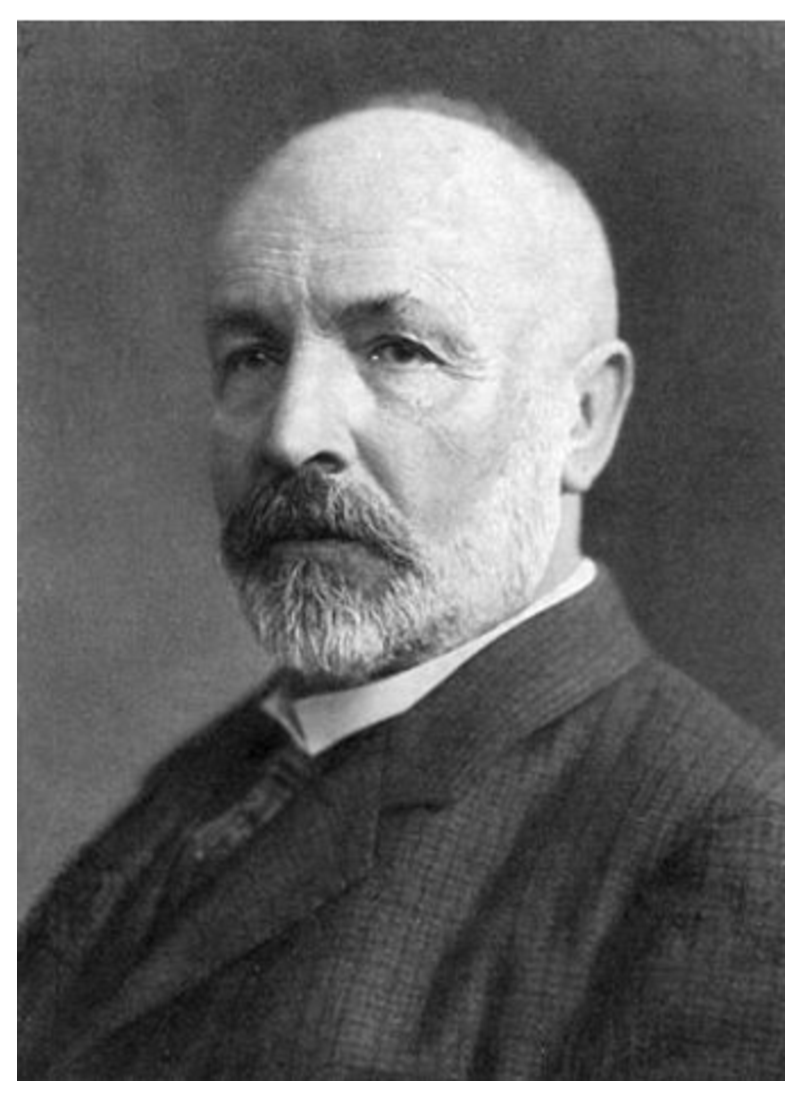
\includegraphics[width=2cm]{Georg-Cantor}}
\noindent\textbf{Georg Cantor} (1845--1918) was born in Saint Petersburg, Russia, where his father was a
successful merchant. Cantor, the oldest of six children, ever regarded as an outstanding violinist, developed his interest in mathematics in his teens. He began his university studies
in Zurich in 1862, but when his father died he left Zurich. He continued his university studies at the University
of Berlin in 1863, where he studied under the eminent mathematicians \underline{Karl Weierstrass} (1815--1897, German mathematician often cited as the ``father of modern analysis''), \underline{Ernst Eduard Kummer} (1810--1893, German mathematician), and \underline{Leopold Kronecker} (1823--1891, German mathematician whose doctrine is ``God made the integers, all else is the work of man.''). He received his doctor's degree in 1867, after having written a dissertation on number theory. Cantor assumed a position at the University of Halle (renamed Martin-Luther-Universit\"{a}t Halle-Wittenberg in 1933) in 1869, where he continued working until his death.
\\
He invented set theory, which has become a fundamental theory in mathematics.
Cantor's theory of \textit{transfinite numbers} was originally regarded as so counter-intuitive---even shocking---that it encountered resistance from mathematical contemporaries such as \underline{Leopold Kronecker} and \underline{Henri Poincar\'{e}} (1854--1912, French mathematician, theoretical physicist, engineer, and philosopher of science) and later from \underline{Hermann Weyl} (1885--1955, a German mathematician, theoretical physicist and philosopher) and \underline{L. E. J. Brouwer} (1881--1966, a Dutch mathematician and philosopher), while \underline{Ludwig Wittgenstein} (1889--1951, an Austrian-British philosopher) raised philosophical objections.
The objections to Cantor's work were occasionally fierce: \underline{Henri Poincar\'{e}} referred to his ideas as a ``grave disease'' infecting the discipline of mathematics, and Leopold Kronecker's public opposition and personal attacks included describing Cantor as a ``scientific charlatan'', a ``renegade'' and a ``corrupter of youth''.
\\
The harsh criticism has been matched by later accolades. In 1904, the Royal Society awarded Cantor its Sylvester Medal (James Joseph Sylvester (1814--1897), an English mathematician who made fundamental contributions to matrix theory, invariant theory, number theory, partition theory, and combinatorics), the highest honor it can confer for work in mathematics. \underline{David Hilbert} (1862--1943, German mathematician) defended Cantor's theory from its critics by declaring:\\
From his paradise that Cantor with us unfolded, we hold our breath in awe; knowing, we shall not be expelled.\\
Cantor married Vally Guttmann in 1874 and had five children. His melancholy temperament was balanced by his wife's happy disposition. Although he received a large inheritance from his father, he was poorly paid as a professor. To mitigate this, he tried to obtain a better-paying position at the University of Berlin but was blocked by Kronecker. Cantor suffered from mental illness (chronic depression or a bipolar disorder) from 1884 to the end of his life, which have been blamed on the hostile attitude of many of his contemporaries. Cantor retired in 1913, living in poverty and suffering from malnourishment during World War I (1914--1918). The public celebration of his 70th birthday was canceled because of the war. He died on January 6, 1918 from a heart attack in the sanatorium where he had spent the final year of his life. In Halle (Saale), where the Martin-Luther-Universit\"{a}t Halle-Wittenberg locates, there is a high school named Georg Cantor Gymnasium that is famous for teaching in mathematics and natural science.}


\textbf{Venn Diagrams}~~Sets can be represented graphically using Venn diagrams (also called primary diagrams, set diagrams or logic diagrams), named after the English mathematician
John Venn \footnote{\parpic{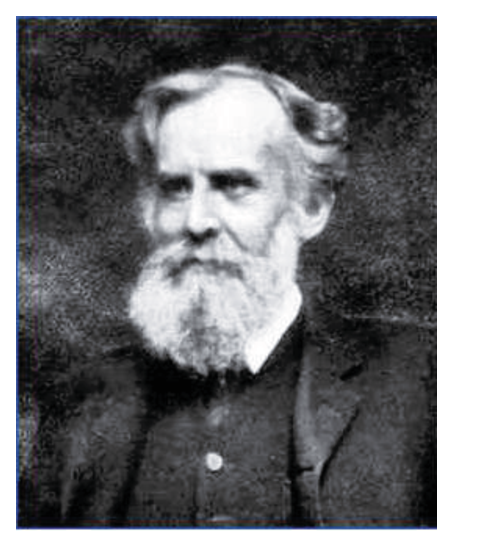
\includegraphics[width=2cm]{Venn}}
\noindent\textbf{John Venn} (1834--1923) was as an English logician and philosopher noted for introducing the Venn diagram, used in the fields of set theory, probability, logic, statistics, and computer science.
\\He began his education in London joining Sir Roger Cholmeley's School, now known as Highgate School, with his brother Henry in September 1846. In 1857, he obtained his degree in mathematics and became a fellow. In 1903 he was elected President of the College, a post he held until his death. In 1862, he returned to Cambridge as a lecturer in moral science, studying and teaching logic and probability theory, and, beginning around 1869, giving intercollegiate lectures. These duties led to his developing the diagram which would eventually bear his name.
\\
Venn built rare machines. The function of the machine was to bowl cricket balls. The machine was so fascinating that when the Australians were visiting Cambridge, the machines were used to entertain them. The bowl cricket ball that Venn built actually bowled out the top ranked player of the team four times consecutively.
\\
Venn was president of the Cambridge Antiquarian Society for 1908-1909. He is also listed as a vice president of the Cambridge Provident Medical Institution. Venn was a prominent supporter of votes for women. He co-signed with his wife Susanna, a letter to the Cambridge Independent Press published 16 October 1908, encouraging women to put themselves forward as candidates for the up-and-coming Cambridge town council elections. The letter was co-sponsored by Lady \underline{Maud Darwin}, wife of Sir \underline{George Darwin} (1845--1912, English barrister and astronomer, born at Down House, Kent, the second son and fifth child of Charles Darwin) and daughter-in-law of \underline{Charles Darwin} (1809--1882, English naturalist, geologist and biologist, best known for his contributions to the science of evolution), plus \underline{Florence Ada Keynes} (1861--1958, female, British author, historian and politician), who would later go on to become the first woman elected to Cambridge Town Council (now Cambridge City Council) and the second woman to become Mayor of Cambridge, in 1932-1933. She's also known for being the mother of the economist \underline{John Maynard Keynes} (1883--1946, British economist whose ideas fundamentally changed the theory and practice of macroeconomics and the economic policies of governments. He built on and greatly refined earlier work on the causes of business cycles, and is widely considered to be one of the most influential economists of the 20th century and the founder of modern macroeconomics theory. His ideas are the basis for the \textit{school of thought} known as \textit{Keynesian economics}, and its various offshoots.).}, who introduced their use in 1881. In Venn diagrams the universal set $U$, which
contains all the objects under consideration, is represented by a rectangle (Note that the universal
set varies depending on which objects are of interest). Inside this rectangle, circles or
other geometrical figures are used to represent sets. Sometimes points are used to represent the
particular elements of the set. Venn diagrams are often used to indicate the relationships between
sets.

\begin{example}
Draw a Venn diagram that represents $V$, the set of vowels in the English alphabet.
We draw a rectangle to indicate the universal set $U$, which is the set of the 26 letters
of the English alphabet. Inside this rectangle we draw a circle to represent $V$. Inside this circle
we indicate the elements of $V$ with points, as seen in Figure \ref{fig1-001}. \hfill$\square$
\end{example}





\begin{figure}[htbp]
%\sidecaption
%\includegraphics[scale=.45]{fig1-001.eps}
%\begin{center}
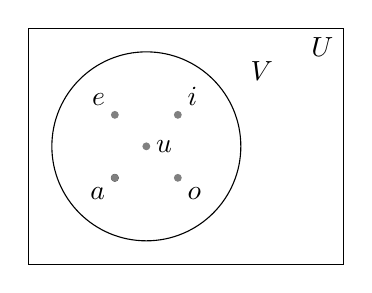
\begin{tikzpicture}
\fill[black] (-0.4,-0.4) circle (0.05cm);
\fill[gray] (-0.4,0.4) circle (0.05cm);
\fill[gray] (-0.4,-0.4) circle (0.05cm);
\fill[gray] (0.4,0.4) circle (0.05cm);
\fill[gray] (0.4,-0.4) circle (0.05cm);
\fill[gray] (0,0) circle (0.05cm);
\draw (0,0) circle (1.2cm);
\draw (-1.5,-1.5) rectangle (2.5,1.5) node [text=black,below left] {$U$};
\draw (-0.4,-0.4) node [text=black,below left] {$a$};
\draw (-0.4,0.4)  node [text=black,above left] {$e$};
\draw (0.4,0.4)   node [text=black,above right] {$i$};
\draw (0.4,-0.4)  node [text=black,below right] {$o$};
\draw (1.2,1.2)   node [text=black,below right] {$V$};
\draw (0,0)       node [text=black,right] {$u$};
\end{tikzpicture}
%\end{center}
\caption{Venn graph for the set of vowels.}
\label{fig1-001}       % Give a unique label
\end{figure}



It is common to encounter situations where the elements of one set are also the elements of
a second set. We now introduce some terminologies and notations to express such relationships
between sets.

\begin{definition}
The set $A$ is a subset of $B$ if and only if every element of $A$ is also an element of $B$. We use
the notation $A\subseteq{B}$ to indicate that $A$ is a subset of the set $B$.
\end{definition}


We see that $A\subseteq B$ if and only if the quantification

\[\forall x(x\in A\Rightarrow{x}\in{B})\]

\noindent is true. Note that to show that $A$ is not a subset of $B$ we need only find one element $x\in{A}$ with
$x\notin{B}$. Such an $x$ is a counterexample to the claim that $x\in{A}$ implies $x\in{B}$.


\begin{example}
The set of all odd positive integers less than 10 is a subset of the set of all positive integers less
than 10, the set of rational numbers is a subset of the set of real numbers, the set of all computer
science majors at your school is a subset of the set of all students at your school, and the set of
all people in China is a subset of the set of all people in China (that is, it is a subset of itself).
Each of these facts follows immediately by noting that an element that belongs to the first set
in each pair of sets also belongs to the second set in that pair.
\hfill$\square$
\end{example}



\begin{example}
The set of integers with squares less than 100 is not a subset of the set of nonnegative integers because -1 is in the former set (as $(-1)^2<100$), but not the later set. The set of people who
have taken discrete mathematics at your school is not a subset of the set of all computer science majors at your school if there is at least one student who has taken discrete mathematics who is
not a computer science major.
\hfill$\square$
\end{example}

Given any nonempty set $S$, it is guaranteed to have at least two subsets, the empty set and the set $S$ itself, that is, $\emptyset\subseteq{S}$ and $S\subseteq{S}$.

When we wish to emphasize that a set $A$ is a subset of a set $B$ but that $A\neq B$, we write
$A\subset{B}$ and say that $A$ is a \textit{proper subset} of $B$. For $A\subset{B}$ to be true, it must be the case that
$A\subseteq{B}$ and there must exist an element $x$ of $B$ that is not an element of $A$. That is, $A$ is a proper
subset of $B$ if and only if

\[\forall x(x\in{A}\Rightarrow x\in{B})\wedge\exists{y}(y\in{B}\wedge y\notin{A})\]


\noindent is true. Venn diagrams can be used to illustrate that a set $A$ is a subset of a set $B$. We draw the
universal set $U$ as a rectangle. Within this rectangle we draw a circle for $B$. Because $A$ is a subset
of $B$, we draw the circle for $A$ within the circle for $B$. This relationship is shown in Figure \ref{fig1-002}.



\begin{figure}[htbp]
%\sidecaption
%\includegraphics[scale=.45]{fig1-002.eps}
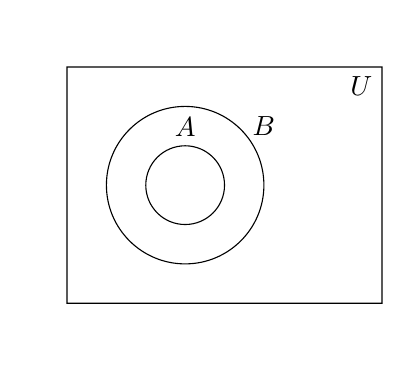
\begin{tikzpicture}[fill=gray]
% left hand
\scope
\clip (-2,-2) rectangle (2,2)
      (1,0) circle (1);
%\fill (0,0) circle (1);
\endscope
% right hand
\scope
\clip (-2,-2) rectangle (2,2)
      (0,0) circle (1);
%\fill (1,0) circle (1);
\endscope
% outline
%\fill[gray] (0,0) circle (0.5);
\draw (0,0) circle (0.5) (0,0.5)  node [text=black,above] {$A$}
      (0,0) circle (1) (1,1)  node [text=black,below] {$B$}
      (-1.5,-1.5) rectangle (2.5,1.5) node [text=black,below left] {$U$};
\end{tikzpicture}
\caption{Venn graph showing that $A$ is a proper subset of $B$.}
\label{fig1-002}       % Give a unique label
\end{figure}





A useful way to show that two sets have the same elements is to show that each set is a subset of the other. In other words, we can show that if $A$ and $B$ are sets with $A\subseteq{B}$ and $B\subseteq{A}$, then $A=B$. That is, $A=B$ if and only if $\forall x(x\in A\Rightarrow x\in{B})$ and $\forall x(x\in{B}\Rightarrow x\in A)$ or
equivalently if and only if $\forall x(x\in{A}\Leftrightarrow x\in{B})$, which is what it means for the $A$ and $B$ to be
equal.

\begin{example}
$A=\{\emptyset, \{a\}, \{b\}, \{a,b\}\}$ and $B=\{x|x~\text{is a subset of the set}~\{a,b\}\}$ are equal.
\hfill$\square$
\end{example}



\textbf{The Size of a Set}~~Sets are used extensively in counting problems, and for such applications we need to discuss
the sizes of sets.

\begin{definition}
Let $S$ be a set. If there are exactly $n$ distinct elements in $S$ where $n$ is a nonnegative integer,
we say that $S$ is a finite set and that $n$ is the cardinality of $S$. The cardinality of S is denoted by $|S|$.
\end{definition}


\begin{example}
Let $A$ be the set of odd positive integers less than 10. Then $|A|=5$. \hfill$\square$
\end{example}

\begin{example}
Let $S$ be the set of letters in the English alphabet. Then $|S|= 26$. \hfill$\square$
\end{example}



\begin{example}
Because the null set has no elements, it follows that $|\emptyset| =0$. \hfill$\square$
\end{example}

A set is said to be \textit{infinite} if it is not finite. For example, the set of all nonnegative integers $\{0, 1, 2, \ldots\}$ is infinite and the set of all even nonnegative numbers $\{0, 2, 4, \ldots\}$ is infinite. It is obvious that $\{0, 2, 4, \ldots\}$ is a proper subset of $\{0, 1, 2, \ldots\}$.
We will extend the notion of cardinality to infinite sets in Section 2.5, which is a challenging topic
full of surprising results \footnote{For a finite set, its cardinality provides an exact measure of its size. However, for infinite sets, the cardinality is a relative measure of two sets. Specifically, we can define what it means for one infinite set to have a small cardinality than another infinite set. The pertinent results regarding this issue are largely attributed to the work of Cantor and Julius Wilhelm Richard Dedekind (1831--1916). A primary surprising result is that sets $A=\{2, 4, 6, \ldots\}$ and $\mathbb{N}^+=\{1, 2, 3, \ldots\}$ have the same cardinality, represented by $|A|=|\mathbb{N}^+|$ (although $A\subset\mathbb{N}^+$ is obviously true). Since the concept of functions is needed to define the cardinality of an infinite set, we leave the problem in Chapter 2.}.


\textbf{Power Sets}~~Many problems involve testing all combinations of elements of a set to see if they satisfy some
property. To consider all such combinations of elements of a set $S$, we build a new set that has
as its members all the subsets of $S$.


\begin{definition}
Given a set $S$, the power set of $S$ is the set of all subsets of the set $S$. The power set of $S$ is
denoted by $\mathcal{P}(S)$.
\end{definition}



\begin{example}
The power set $\mathcal{P}(\{0, 1, 2\})$ is the set of all subsets of \{0, 1, 2\}. Hence,
$\mathcal{P}(\{0, 1, 2\})=\{\emptyset, \{0\}, \{1\}, \{2\}, \{0, 1\}, \{0, 2\}, \{1, 2\}, \{0, 1, 2\}\}$.
\hfill$\square$
\end{example}


\begin{example}
We have $\mathcal{P}(\emptyset)=\{\emptyset\}$ and $\mathcal{P}(\{\emptyset\})=\{\emptyset, \{\emptyset\}\}$.
\hfill$\square$
\end{example}

\begin{remark}
If a set $A$ has $n$ (disctinct) elements, then its power set contains $2^n$ members. Accordingly, sometimes $\mathcal{P}$ is written as $2^A$. \hfill$\square$
\footnote{\parpic{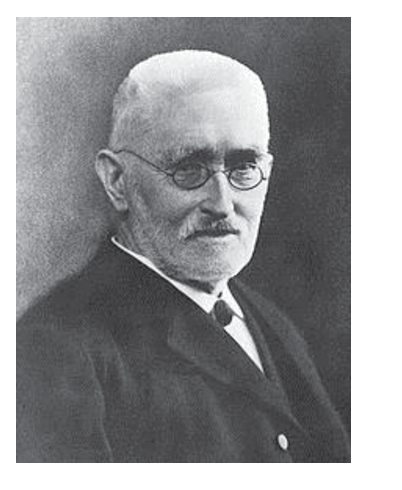
\includegraphics[width=2.0cm]{Dedekind.eps}}\noindent Julius Wilhelm Richard Dedekind (1831--1916) was a German mathematician who made important contributions to abstract algebra (particularly ring theory), algebraic number theory and the definition of the real numbers.\\
He was born, lived most of his life, and died in Braunschweig (often called ``Brunswick'' in English).
He first attended the Collegium Carolinum in 1848 before transferring to the University of G\"{o}ttingen in 1850. There, Dedekind was taught number theory by Professor Moritz Stern and he became Gauss's last student there. Dedekind received his doctorate in 1852. The thesis however did not display the talent evident by his subsequent work.\\
Dedekind went to Berlin for two years of study, where he and Bernhard Riemann (1826--1866, a German mathematician who made contributions to analysis, number theory, and differential geometry) were contemporaries; they were both awarded the habilitation in 1854. Dedekind returned to G\"{o}ttingen to teach, giving courses on probability and geometry. He studied for a while with Peter Gustav Lejeune Dirichlet (1805--1859, a German mathematician who made deep contributions to number theory, Fourier series and other topics in mathematical analysis, credited with being one of the first mathematicians to give the modern formal definition of a function), and they became good friends.
\\
Dedekind developed the notion now known as a Dedekind cut, now a standard definition of the real numbers.
In 1888, he published a short monograph titled ``What are numbers and what should they be?'' which included his definition of an infinite set. He also proposed an axiomatic foundation for the natural numbers, whose primitive notions were the number one and the successor function. In 1872, while on holiday in Interlaken, Dedekind met Georg Cantor. Thus they began an enduring relationship of mutual respect, and Dedekind became one of the very first mathematicians to admire Cantor's work concerning infinite sets, proving a valued ally in Cantor's disputes with Leopold Kronecker, who was philosophically opposed to Cantors's transfinite numbers.\\
He retired in 1894, but did occasional teaching and continued to publish. He never married, instead living with his sister Julia.
Dedekind was elected to the Academies of Berlin (1880) and Rome, and to the French Academy of Sciences (1900). He received honorary doctorates from the universities of Oslo, Zurich, and Braunschweig.\\
Interestingly and accidentally, Johann Carl Friedrich Gauss (1777--1855, a German mathematician who contributed significantly to many fields, including number theory, algebra, statistics, analysis, differential geometry, geodesy, geophysics, mechanics, electrostatics, astronomy, matrix theory, and optics, referred to as ``the foremost of mathematicians'' and ``greatest mathematician since antiquity''. Gauss had an exceptional influence in many fields of mathematics and science and is ranked as one of history's most influential mathematicians) was also born in the small town Braunschweig (252,768 people, as of 31 December 2015), where the residents are all proud of the two mathematicians.\\
There is an anecdote regarding the death of Dedekind. He lived so long that although some of his work had been familiar to all the students of analysis for a generation before his death, he himself had become almost a legend and many classed him with the shadowy dead. Twelve years before his death, a book \textit{Calendar for Mathematicians} listed Dedekind as having died on September 4, 1899, much to Dedekind's amusement. The day, September 4, might possible prove to be correct, he wrote to the editor of the book, but the year was certainly wrong.  `According to my memorandum I passed this day in perfect health and enjoyed a very stimulating conversation on ``system and theory'' with my luncheon guest and honoured friend Georg Cantor of Halle.'}
\end{remark}

\begin{remark}
For a finite non-empty set $A$, it is rather intuitive that the cardinality of set $A$ is strictly less than that of its power set $2^A$ or $\mathcal{P}(A)$, i.e., $|A|<|\mathcal{P}(A)|$. When $A$ is infinite, $\mathcal{P}(A)$ is naturally infinite. The relative measure of $|A|$ and $|\mathcal{P}(A)|$ is important for mathematics analysis. \hfill$\square$
\end{remark}


\textbf{Cartesian Products}~~The order of elements in a collection is often important. Because sets are unordered, a different
structure is needed to represent ordered collections. This is provided by \textbf{ordered $n$-tuples}.

\begin{definition}
An ordered $n$-tuple $(a_1, a_2, \ldots, a_n)$ is the ordered collection that has $a_1$ as its first element,
$a_2$ as its second element, $\ldots$, and $a_n$ as its $n$-th element.
\end{definition}

We say that two ordered $n$-tuples are equal if and only if each corresponding pair of their
elements is equal. In other words, $(a_1, a_2, \ldots, a_n)=(b_1, b_2, \ldots, b_n)$ if and only if $a_i=b_i$,
for $i=1, 2, \ldots, n$. In particular, ordered 2-tuples are called ordered pairs. The ordered pairs
$(a, b)$ and $(c, d)$ are equal if and only if $a=c$ and $b=d$. Note that $(a, b)$ and $(b, a)$ are not
equal unless $a=b$.

Many of the discrete structures are based on the notion of the
Cartesian product of sets (named after Ren\'{e} Descartes). We first define the Cartesian product
of two sets \footnote{\parpic{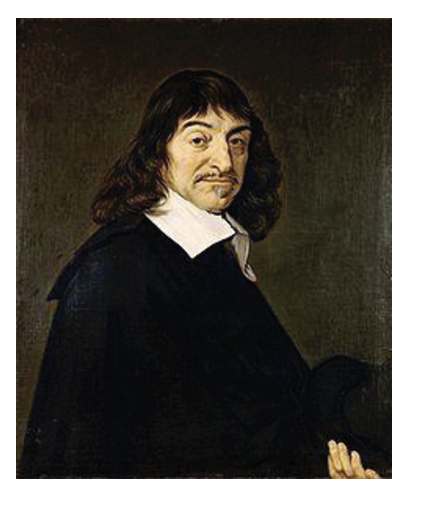
\includegraphics[width=2cm]{Descartes.eps}}\noindent Ren\'{e} Descartes (1596--1650) was a French philosopher, mathematician, and scientist. Dubbed the father of modern western philosophy, much of subsequent Western philosophy is a response to his writings, which are studied closely to this day.\\
Descartes was born into a noble family near Tours, France, about
200 miles southwest of Paris. He was the third child of his father's first wife. When he was one year old, his mother Jeanne Brochard died after trying to give birth to another child who also died. Because of Ren\'{e}'s poor health, his father, a provincial judge, let his son's formal lessons slide until, at
the age of 8, Ren\'{e} entered the Jesuit college at La Fl\`{e}che. The rector of the school took a liking to him and
permitted him to stay in bed until late in the morning because of his frail health. From then on, Descartes spent
his mornings in bed; he considered these times his most productive hours for thinking.\\
Descartes left school in 1612, moving to Paris, where he spent 2 years studying mathematics. He earned
a law degree in 1616 from the University of Poitiers. At 18 Descartes became disgusted with studying and
decided to see the world. He moved to Paris and became a successful gambler. However, he grew tired
of bawdy living and moved to the suburb of Saint-Germain, where he devoted himself to mathematical study. When his gambling
friends found him, he decided to leave France and undertake a military career. However, he never did any fighting. One day, while
escaping the cold in an overheated room at a military encampment, he had several feverish dreams, which revealed his future career as a mathematician and philosopher.\\
After ending his military career, he traveled throughout Europe. He then spent several years in Paris, where he studied mathematics and philosophy and constructed optical instruments. Descartes decided to move to Holland, where he spent 20 years wandering around the country, accomplishing his most important work. During this time he wrote several books, including the \textit{Discours}, which contains his contributions to analytic geometry, for which he is best known. He also made fundamental contributions to philosophy. \\
In 1649 Descartes was invited by Queen Christina to visit her court in Sweden to tutor her in philosophy. Although he was
reluctant to live in what he called ��the land of bears amongst rocks and ice,�� he finally accepted the invitation and moved to Sweden. Unfortunately, the winter of 1649--1650 was extremely bitter. Descartes caught pneumonia and died in mid-February.\\
One of Descartes' most enduring legacies was his development of Cartesian or analytic geometry, which uses algebra to describe geometry. He invented the convention of representing unknowns in equations by $x$, $y$, and $z$, and knowns by $a$, $b$, and $c$. He also pioneered the standard notation that uses superscripts to show the powers or exponents, e.g., $x^3$.
\\Current opinion is that Descartes had the most influence of anyone on the young Newton, and this is arguably one of Descartes' most important contributions. Newton continued Descartes' work on cubic equations, which freed the subject from the fetters of the Greek perspectives. Descartes' work provided the basis for the \textit{calculus} developed by Isaac Newton (1642--1726) and Gottfried Leibniz (1646--1716), who applied infinitesimal calculus to the tangent line problem, thus permitting the evolution of that branch of modern mathematics.}.



\begin{definition}
Let $A$ and $B$ be sets. The Cartesian product of $A$ and $B$, denoted by $A\times{B}$, is the set of all
ordered pairs $(a, b)$, where $a\in{A}$ and $b\in{B}$, i.e.,

\[A\times{B}=\{(a, b)|a\in A\wedge b\in B\}.\]
\end{definition}


\begin{example}
Let $A$ represent the set of all students at a university, and let $B$ represent the set of all courses
offered at the university. The Cartesian product $A\times{B}$ consists of all the ordered pairs of the form $(a, b)$, where
$a$ is a student at the university and $b$ is a course offered at the university. One way to use the set
$A\times{B}$ is to represent all possible enrollments of students in courses at the university.
\hfill$\square$
\end{example}


\begin{example}
Let $A=\{1, 2\}$ and $B=\{a, b, c\}$. The Cartesian product $A\times{B}$ is
$A\times{B}=\{(1, a), (1, b), (1, c), (2, a), (2, b), (2, c)\}$.
\hfill$\square$
\end{example}


If any of $A$ and $B$ is empty, $A\times{B}=B\times{A}=\emptyset$. However, in general, $A\times{B}\neq{B\times{A}}$ unless $A=B$. The Cartesian product of more than two sets can also be defined.

\begin{definition}
The Cartesian product of the sets $A_1$, $A_2$, $\ldots$, $A_n$, denoted by $A_1\times{A_2}\times\ldots\times{A_n}$, is the
set of ordered $n$-tuples $(a_1, a_2, \ldots, a_n)$, where $a_i$ belongs to $A_i$ for $i=1, 2, \ldots, n$. In other
words,

\[A_1\times A_2\times\ldots\times A_n=\{(a_1, a_2, \ldots, a_n)|a_i\in A_i~\text{for}~i=1,2, \ldots, n\}.\]
\end{definition}


\begin{example}
Let $A=\{0, 1\}, B=\{1, 2\}$, and $C=\{0, 1, 2\}$. $A\times{B}\times{C}$ consists of all ordered triples $(a, b, c)$, where $a\in{A}$, $b\in{B}$, and $c\in{C}$. Hence,

$A\times{B}\times{C}=\{(0, 1, 0), (0, 1, 1), (0, 1, 2), (0, 2, 0), (0, 2, 1), (0, 2, 2)$, $(1$, $1$, $0)$, $(1$, $1$, $1)$, $(1$, $1, 2), (1, 2, 0), (1, 2, 1), (1, 2, 2)\}.$
\hfill$\square$
\end{example}


We use the notation $A^2$ to denote $A\times{A}$, the Cartesian product of the set $A$ with itself.
Similarly, $A^3=A\times{A}\times{A}$, $A^4=A\times{A}\times{A}\times{A}\times{A}$, and so on. More generally,

\[A^n =\{(a_1, a_2, \ldots, a_n) | a_i\in A~\text{for}~i=1, 2, \ldots, n\}.\]


\begin{example}
Let $A=\{1, 2\}$ be a set. It follows that $A^2=\{(1, 1), (1, 2), (2, 1), (2, 2)\}$ and $A^3=\{(1, 1, 1), (1, 1, 2), (1, 2, 1), (1, 2, 2), (2, 1, 1), (2, 1, 2), (2, 2, 1), (2, 2, 2)\}$.
\hfill$\square$
\end{example}


A subset $R$ of the Cartesian product $A\times{B}$ is called a relation \footnote{\textit{Relation} is an important concept in discrete mathematics, which will be introduced in Chapter 3.} from the set $A$ to the set
$B$. The elements of $R$ are ordered pairs, where the first element belongs to $A$ and the second
to $B$. For example, $R=\{(a, 0), (a, 1), (a, 3), (b, 1), (b, 2), (c, 0), (c, 3)\}$ is a relation from the
set $\{a, b, c\}$ to the set $\{0, 1, 2, 3\}$. A relation from a set $A$ to itself is called a relation on $A$.


Suppose that $A$=\{G88\} and $B$=\{Xian, Zhengzhou, Hebi, Xingtai, Shijiazhuang, Baoding, Beijing\}. Then $R$=\{(G88, Xian), (G88, Zhengzhou), (G88, Shijiazhuang), (G88, Beijing)\} is a relation from $A$ to $B$, indicating the cites in which High Speed Rail G88 (China Railway Corporation) stops over.

\begin{example}
Let $A=\{0,1,2,3\}$ and $R=\{(a,b)|a\leq{b}\}$ be a relation on $A$. Then
$R=\{(0,0)$, $(0,1), (0,2), (0,3), (1,1), (1,2), (1,3),
(2,2), (2, 3), (3, 3)\}$. \hfill$\square$
\end{example}

\section{Set Operations}

Two, or more, sets can be combined in many different ways. For instance, starting with the set
of mathematics majors at your school and the set of computer science majors at your school, we
can form the set of students who are mathematics majors or computer science majors, the set of
students who are joint majors in mathematics and computer science, the set of all students not
majoring in mathematics, and so on.

\begin{definition}
Let $A$ and $B$ be sets. The union of the sets $A$ and $B$, denoted by $A\cup{B}$, is the set that contains
those elements that are either in $A$ or in $B$, or in both.
\end{definition}

An element $x$ belongs to the union of the sets $A$ and $B$ if and only if $x$ belongs to $A$ or $x$ belongs
to $B$. This tells us that

\[A\cup B=\{x|x\in{A}\vee x\in{B}\}.\]


The Venn diagram shown in Figure \ref{union of two sets} represents the union of two sets $A$ and $B$. The area
that represents $A\cup{B}$ is the shaded area within either the circle representing $A$ or the circle
representing $B$.

\begin{figure}[htbp]
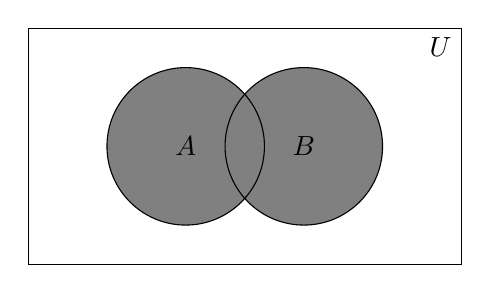
\begin{tikzpicture}
\draw (-2,-1.5) rectangle (3.5,1.5) node[below left]{$U$};
\fill[gray] (0,0) circle (1cm);
\fill[gray] (1.5,0) circle (1cm);
\draw (0,0) circle (1cm) node {$A$};
\draw (1.5,0) circle (1cm) node {$B$};
\end{tikzpicture}
\caption{Venn graph of the union of two sets.}
\label{union of two sets}
\end{figure}

\begin{example}
The union of the sets \{1, 3, 5\} and \{1, 2, 3\} is the set \{1, 2, 3, 5\}; that is,
\{1, 3, 5\}$\cup$\{1, 2, 3\}=\{1, 2, 3, 5\}.
\hfill$\square$
\end{example}


\begin{example}
The union of the sets $\{a, b, c, d\}$ and $\{1, 2, b, d, e\}$ is the set $\{1$, $2$, $a$, $b$, $c$, $d$, $e\}$.
\hfill$\square$
\end{example}

\begin{example}
The union of the set of all computer science majors at Xidian University and the set of all mathematics
majors at Xidian University is the set of students at Xidian University who are majoring either in
mathematics or in computer science (or in both).
\hfill$\square$
\end{example}


\begin{definition}
Let $A$ and $B$ be sets. The \textit{intersection} of the sets $A$ and $B$, denoted by $A\cap{B}$, is the set
containing those elements in both $A$ and $B$.
\end{definition}

An element $x$ belongs to the intersection of the sets $A$ and $B$ if and only if $x$ belongs to $A$ and
$x$ belongs to $B$. This tells us that

\[A\cap{B}=\{x|x\in A\wedge x\in B\}.\]



The Venn diagram shown in Figure \ref{intersection of two sets} represents the intersection of two sets $A$ and $B$. The shaded
area that is within both the circles representing the sets $A$ and $B$ is the area that represents the
intersection of $A$ and $B$.

\begin{figure}[htbp]
%\begin{center}
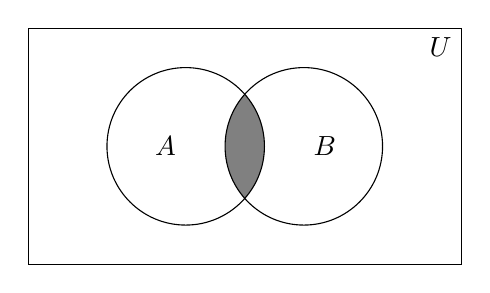
\begin{tikzpicture}
\draw (-2,-1.5) rectangle (3.5,1.5) node[below left]{$U$};
\begin{scope} % start of clip scope
\clip (0,0) circle (1cm);
\fill[gray] (1.5,0) circle (1cm);
\end{scope} % end of clip scope
\draw (0,0) circle (1cm) node[left] {$A$};
\draw (1.5,0) circle (1cm) node[right] {$B$};
\end{tikzpicture}
%\end{center}
\caption{Venn graph of the intersection of two sets.}
\label{intersection of two sets}
\end{figure}


\begin{example}
The intersection of the sets \{1, 3, 5\} and \{1, 2, 3\} is the set \{1, 3\}; that is,
$\{1, 3, 5\}\cap\{1, 2, 3\} = \{1, 3\}$.
\hfill$\square$
\end{example}


\begin{example}
The intersection of the set of all computer science majors at your school and the set of all
mathematics majors is the set of all students who are joint majors in mathematics and computer
science.
\hfill$\square$
\end{example}



We are often interested in finding the cardinality of a union of two finite sets $A$ and $B$. Note that $|A|+|B|$ counts each element that is in $A$ but not in $B$ or in $B$ but not in $A$ exactly once, and each element that is in both $A$ and $B$ exactly twice. Thus, if the number of elements that
are in both $A$ and $B$ is subtracted from $|A|+|B|$, elements in $A\cap B$ will be counted only once. Hence,

\[|A\cup B|=|A|+|B|-|A\cap B|.\]


\begin{definition}
Two sets are said to be \textit{disjoint} if their intersection is the empty set.
\hfill$\square$
\end{definition}


\begin{example}
Let $A=\{1, 3, 5, 7, 9\}$ and $B=\{2, 4, 6, 8, 10\}$. Because $A\cap B=\emptyset$, $A$ and $B$ are disjoint.
\hfill$\square$
\end{example}


\begin{definition}
Let $A$ and $B$ be sets. The \textit{difference} of $A$ and $B$, denoted by $A-B$ or $A\setminus{B}$, is the set containing those
elements that are in $A$ but not in $B$. The difference of $A$ and $B$ is also called the \textit{complement} of $B$ with respect to $A$.
\end{definition}

An element $x$ belongs to the difference of $A$ and $B$ if and only if $x\in A$ and $x\notin{B}$. This tells us
that

\[A-B=\{x|x\in A\wedge x\notin B\}.\]


The Venn diagram shown in Figure \ref{Difference of two sets} represents the difference of the sets $A$ and $B$. The shaded
area inside the circle that represents $A$ and outside the circle that represents $B$ is the area that
represents $A-B$.


\begin{figure}[htbp]
%\begin{center}
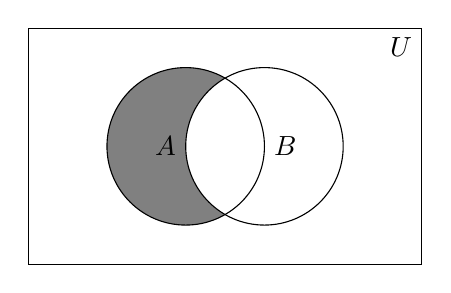
\begin{tikzpicture}
\draw (-2,-1.5) rectangle (3,1.5) node[below left]{$U$}; % draw a rectangle
\fill[gray] (0,0) circle (1cm); % then fill in a circular region
\fill[white] (1,0) circle (1cm); % then fill in a 2nd circular region
\draw (0,0) circle (1cm) node[left] {$A$};
\draw (1,0) circle (1cm) node[right] {$B$};
\end{tikzpicture}
%\end{center}
\caption{Venn graph of the difference of two sets.}
\label{Difference of two sets}
\end{figure}


\begin{example}
The difference of \{1, 3, 5\} and \{1, 2, 3\} is the set \{5\}; that is, $\{1, 3, 5\}-\{1, 2, 3\}=\{5\}$. This
is different from the difference of \{1, 2, 3\} and \{1, 3, 5\}, which is the set \{2\}.
\hfill$\square$
\end{example}

\begin{example}
The difference of the set of computer science majors at your school and the set of mathematics majors at your school is the set of all computer science majors at your school who are not also
mathematics majors.
\hfill$\square$
\end{example}



Once the universal set $U$ has been specified, the complement of a set can be defined.


\begin{definition}
Let $U$ be the universal set. The \textit{complement} of the set $A$, denoted by $\overline{A}$, is the complement
of $A$ with respect to $U$. Therefore, the complement of the set A is $U-A$.
\end{definition}

An element belongs to $\overline{A}$ if and only if $x\notin{A}$. This tells us that

\[\overline{A}=\{x\in U|x\notin A\}.\]


In Figure \ref{complement of a set} the shaded area outside the circle representing $A$ is the area representing $\overline{A}$.

\begin{figure}[htbp]
\begin{center}
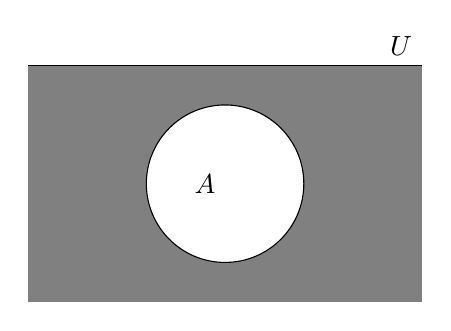
\begin{tikzpicture}
\draw (-2,-1.5) rectangle (3,1.5) node[above left] {$U$}; % draw a rectangle
\fill[gray] (-2,-1.5) rectangle (3,1.5); % then fill in a circular region
\fill[white] (0.5,0) circle (1cm); % then fill in a 2nd circular region
\draw (0.5,0) circle (1cm) node[left] {$A$};
\end{tikzpicture}
\caption{Venn diagram of the complement of a set.}
\label{complement of a set}
\end{center}
\end{figure}

\begin{example}
Let $A=\{a, e, i, o, u\}$ (where the universal set is the set of letters of the English alphabet). Then
$\overline{A}=\{b, c, d, f, g, h, j, k, l, m, n, p, q, r, s, t, v, w, x, y, z\}$.
\hfill$\square$
\end{example}


\begin{example}
Let $A$ be the set of positive integers greater than 10 (with universal set the set of all positive
integers). Then $\overline{A}=\{1, 2, 3, 4, 5, 6, 7, 8, 9, 10\}$.
\hfill$\square$
\end{example}


\textbf{Set Identities}~~
Table \ref{set identities} lists the most important set identities. We can prove these identities
using different methods. These methods are presented to illustrate that there are often many
different approaches to the solution of a problem. The proofs of the remaining identities will
\marginpar{\small Set identities and propositional equivalences are just special cases of identities
for Boolean algebra.}
be left as exercises. The reader should note the similarity between these set identities and the
logical equivalences. In fact, the set identities given can be proved directly from the corresponding logical equivalences.
Furthermore, both are special cases of identities that hold for Boolean algebra.

\begin{table}
\caption{Set identities}
\begin{tabular}{|p{8cm}||p{3cm}|}
  \hline
  Identity & Name\\
  \hline
  $A\cap{U}=A$, $A\cup\emptyset=A$ & Identity laws \\
  \hline
  $A\cup{U}=U$, $A\cap\emptyset=\emptyset$ & Domination laws \\
  \hline
  $A\cup{A}=A$, $A\cap{A}=A$ & Idempotent laws \\
  \hline
  $\overline{(\overline{A})}=A$ & Complementation law \\
  \hline
  $A\cup{B}=B\cup{A}$, $A\cap{B}=B\cap{A}$ & Commutative laws \\
  \hline
  $A\cup{(B\cup C)}=(A\cup B)\cup{C}$, $A\cap{(B\cap C)}=(A\cap{B})\cap{C}$ & Associative laws \\
  \hline
  $A\cup(B\cap C)=(A\cup B)\cap(A\cup C)$, $A\cap (B\cup C)=(A\cap B)\cup(A\cap C)$ & Distributive laws \\
  \hline
  $\overline{A\cap B}=\overline{A}\cup\overline{B}$, $\overline{A\cup{B}}=\overline{A}\cap\overline{B}$ & De Morgan's laws\\
    \hline
  $A\cup(A\cap B)=A$, $A\cap(A\cup B)=A$ & Absorption laws \\
  \hline
  $A\cup\overline{A}=U$, $A\cap\overline{A}=\emptyset$ & Complement laws \\
  \hline
\end{tabular}
\label{set identities}
\end{table}

One way to show that two sets are equal is to show that each is a subset of the other. Recall
that to show that one set is a subset of a second set, we can show that if an element belongs to
the first set, then it must also belong to the second set. We generally use a direct proof to do this.
We illustrate this type of proof by establishing the first of De Morgan's laws.



\begin{example}
Prove that $\overline{(A\cap B)}=\overline{A}\cup\overline{B}$.

Solution: First, we will show that $\overline{A\cap B}\subseteq\overline{A}\cup\overline{B}$. We do this by showing that if $x$ is in $\overline{A\cap B}$, then it must also be in $\overline{A}\cup\overline{B}$. Now suppose that $x\in\overline{A\cap B}$. By the definition of complement, $x\notin A\cap B$. Using the definition of intersection, we see that the proposition $\neg((x\in A) \wedge(x\in B))$ is true.

By applying De Morgan's law for propositions, we see that $\neg(x\in A)$ or $\neg(x\in B)$. Using
the definition of negation of propositions, we have $x\notin A$ or $x\notin B$. Using the definition of
the complement of a set, we see that this implies that $x\in\overline{A}$ or $x\in\overline{B}$. Consequently, by the
definition of union, we see that $x\in\overline{A}\cup\overline{B}$. We have now shown that $\overline{A\cap B}\subseteq\overline{A}\cup\overline{B}$.

Next, we will show that $\overline{A}\cup\overline{B}\subseteq\overline{A\cap B}$. We do this by showing that if $x$ is in $\overline{A}\cup\overline{B}$, then it must also be in $\overline{A\cap B}$. Now suppose that $x\in\overline{A}\cup\overline{B}$. By the definition of union, we know that
$x\in\overline{A}$ or $x\in\overline{B}$. Using the definition of complement, we see that $x\notin A$ or $x\notin B$. Consequently, the proposition $\neg(x\in A)\vee\neg(x\in B)$ is true.

By De Morgan's law for propositions, we conclude that $\neg((x\in A)\wedge(x\in B))$ is true.
By the definition of intersection, it follows that $\neg(x\in A\cap B)$. We now use the definition of
complement to conclude that $x\in\overline{A\cap B}$. This shows that $\overline{A}\cup\overline{B}\subseteq\overline{A\cap B}$.

Because we have shown that each set is a subset of the other, the two sets are equal, and the identity is proved. \marginpar{\small Mathematical induction, a form of direct proof, is a mathematical proof technique used to prove a given statement about any well-ordered set.} \footnote{\parpic{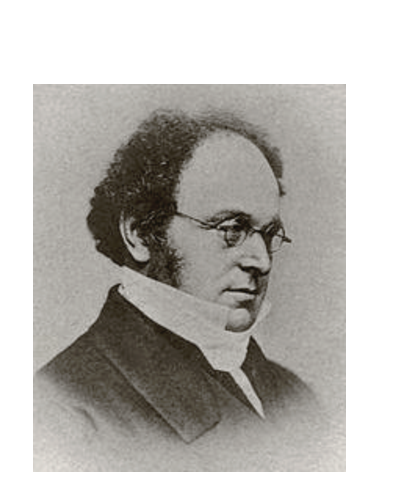
\includegraphics[width=2.0cm]{Morgan.eps}}Augustus De Morgan (1806--1871) was a British mathematician and logician. He formulated De Morgan's laws and introduced the term mathematical induction, making its idea rigorous. In his own time he was better known as a newspaper columnist.\\
De Morgan studied at Trinity College, Cambridge, graduating in 1827. Although he considered medicine or law, he decided on
mathematics for his career. In the 1840s De Morgan made fundamental contributions to the development of symbolic logic. He invented notations that helped him prove propositional equivalences, such as the laws that are named after him. In 1842 De Morgan presented what is considered to be the first precise definition of a limit and developed new tests for convergence of infinite series. De Morgan was also interested in the history of mathematics and wrote biographies of \underline{Newton} and \underline{Halley} (1656--1742, an English astronomer, geophysicist, mathematician, meteorologist, and physicist who is best known for computing the orbit of Halley's Comet).
\\
De Morgan was famous for his opposition to negative numbers, which nowadays flabbergasts our contemporaries since, without thinking too much about it, most of us can use negative numbers for things like recording temperatures below zero and representing economy recession by negative increase. It takes a long time until the end of the 19th century that negative numbers are well accepted by the community of mathematics as part of the number system. \\
Although the first set of rules for dealing with negative numbers was stated in the 7th century by the Indian mathematician Brahmagupta, it is surprising that in 1758 the British mathematician \underline{Francis Maseres} (1731--1824, an English lawyer, known as attorney general of the Province of Quebec, judge, mathematician, historian, and member of the Royal Society) was claiming that negative numbers\\
``\ldots\ldots darken the very whole doctrines of the equations and make dark of the things which are in their nature excessively obvious and simple''.\\
In the early work solving equations, negative roots were not even considered. Hindu mathematicians in the sixth century, and before that, Chinese mathematicians figured out all the rules for operations with negative numbers. Yet the Arabs did not include any of this in their work three centuries later. French mathematician \underline{Blaise Pascal} (1623-1662, a French mathematician, physicist, inventor, writer and Catholic theologian) did not see the need for negative numbers. De Morgan thought numbers less than zero were unimaginable. \\For females, De Morgan cautioned them against
studying too much mathematics, because it might interfere with their childbearing abilities.}
\hfill$\square$
\label{set identity 1}
\end{example}


We can more succinctly express the reasoning used in Example \ref{set identity 1} using set builder notation,
as Example \ref{set identity 2} illustrates

\begin{example}
Use set builder notation and logical equivalences to establish the first De Morgan law $\overline{A\cap B}=
\overline{A}\cup\overline{B}$.

Solution: We can prove this identity with the following steps.

$\overline{A\cap{B}}=\{x|x\notin A\cap{B}\}$ \hfill by definition of complement

$=\{x|\neg(x\in(A\cap B))\}$ \hfill by definition of ``does not belong symbol''

$=\{x|\neg(x\in A\wedge x\in B)\}$ \hfill by definition of intersection

$=\{x |\neg(x\in A)\vee\neg(x\in B)\}$ \hfill by the second De Morgan law

\hfill for logical equivalences
\marginpar{De Morgan's law for logical equivalence is $\neg(p\wedge q)=\neg p\vee\neg q$ and $\neg(p\vee q)=\neg p\wedge\neg q$, where $p$ and $q$ are propositions.}


$=\{x|x\notin A\vee\notin B\}$ \hfill by definition of ``does not belong symbol''

$=\{x|x\in\overline{A}\vee x\in\overline B\}$ \hfill by definition of complement

$=\{x|x\in\overline{A}\cup\overline{B}\}$ \hfill by definition of union

$=\overline{A}\cup\overline{B}$ \hfill by meaning of set builder notation

Note that besides the definitions of complement, union, set membership, and set builder
notation, this proof uses the second De Morgan law for logical equivalences.
\hfill$\square$
\label{set identity 2}
\end{example}


\begin{example}
Prove the second distributive law from Table 1, which states that
$A\cap (B\cup C)=(A\cap B)\cup (A\cap C)$ for all sets $A$, $B$, and $C$.


Solution: We will prove this identity by showing that each side is a subset of the other side.
Suppose that $x\in A\cap(B\cup C)$. Then $x\in A$ and $x\in B\cup C$. By the definition of union, it
follows that $x\in A$, and $x\in B$ or $x\in C$ (or both). In other words, we know that the compound
proposition $(x\in A)wedge((x\in B)\vee(x\in C))$ is true. By the distributive law for conjunction over
disjunction, it follows that $((x\in A)\wedge(x\in B))\vee((x\in A)\wedge(x\in C))$. We conclude that either
$x\in A$ and $x\in B$, or $x\in A$ and $x\in C$. By the definition of intersection, it follows that $x\in A\cap B$
or $x\in A\cap C$. Using the definition of union, we conclude that $x\in (A\cap B)\cup(A\cap C)$. We
conclude that $A\cap(B\cup C)\subseteq(A\cap B)\cup(A\cap C)$.


Now suppose that $x\in(A\cap B)\cup(A\cap C)$. Then, by the definition of union, $x\in A\cap B$ or
$x\in A\cap C$. By the definition of intersection, it follows that $x\in A$ and $x\in B$ or that $x\in A$ and
$x\in C$. From this we see that $x\in A$, and $x\in B$ or $x\in C$. Consequently, by the definition of
union we see that $x\in A$ and $x\in B\cup C$. Furthermore, by the definition of intersection, it follows
that $x\in A\cap (B\cup C)$. We conclude that $(A\cap B)\cup(A\cap C)\subseteq A\cap(B\cup C)$. This completes
the proof of the identity.
\hfill$\square$
\end{example}


Because unions and intersections of sets satisfy associative laws, the sets $A\cup B\cup C$ and
$A\cap B\cap C$ are well defined; that is, the meaning of this notation is unambiguous when $A$,
$B$, and $C$ are sets. That is, we do not have to use parentheses to indicate which operation
comes first because $A\cup(B\cup C)=(A\cup B)\cup C$ and $A\cap(B\cap C)=(A\cap B)\cap C$. Note that
$A\cup B\cup C$ contains those elements that are in at least one of the sets $A$, $B$, and $C$, and that
$A\cap B\cap C$ contains those elements that are in all of $A$, $B$, and $C$.


\begin{example}
Let $A=\{0, 2, 4, 6, 8\}$, $B=\{0, 1, 2, 3, 4\}$, and $C=\{0, 3, 6, 9\}$. The set $A\cup B\cup C$ contains those elements in at least one of $A$, $B$, and $C$. Hence, $A\cup B\cup C=\{0, 1, 2, 3, 4, 6, 8, 9\}$.
The set $A\cap B\cap C$ contains those elements in all three of $A$, $B$, and $C$. Thus, $A\cap B\cap C=\{0\}$.
\hfill$\square$
\end{example}




\begin{definition}
The union of a collection of sets is the set that contains those elements that are members of
at least one set in the collection.
\end{definition}

We use the notation

\[A_1\cup A_2\cup\ldots\cup A_n=\cup_{i=1}^{n}A_i\]

\noindent to denote the union of the sets $A_1$, $A_2$, $\ldots$, $A_n$.

\begin{definition}
The intersection of a collection of sets is the set that contains those elements that are members
of all the sets in the collection.
\end{definition}

We use the notation

\[A_1\cap A_2\cap\ldots\cap A_n=\cap_{i=1}^{n}A_i\]

\noindent to denote the intersection of the sets $A_1$, $A_2$, $\ldots$, $A_n$.


\begin{example}
For $i=1, 2, \ldots$, let $A_i=\{i, i + 1, i + 2, \ldots\}$. Then,


\[\cup_{i=1}^{n}A_i=\cup_{i=1}^{n}\{i, i+1, i+2, \ldots\}=\{1, 2, 3, \ldots\},\]

and

\[\cap_{i=1}^{n}A_i=\cap_{i=1}^{n}\{i, i+1, i+2, \ldots\}=\{n, n+1, n+2, \ldots\}=A_n.\]
\hfill$\square$
\end{example}


\begin{definition}
Let $A_1$, $A_2$, $\ldots$, $A_n$ be subsets of $S$. $A_1$, $A_2$, $\ldots$, $A_n$ are said to be a partition of $S$ if (1) $\cup_{i=1}^{n}A_i=S$ and (2) $\forall i\neq{j}$ $(i,j\in\mathbb{N}_n)$, $A_i\cap{A_j}=\emptyset$.
\end{definition}



\begin{example}
Consider the following collections of subsets of $S=\{1, 2, . . ., 8, 9\}$:

(i) \{1, 3, 5\}, \{2, 6\}, \{4, 8, 9\};

(ii) \{1, 3, 5\}, \{2, 4, 6, 8\}, \{5, 7, 9\}; and

(iii) \{1, 3, 5\}, \{2, 4, 6, 8\}, \{7, 9\}.

It is trivial that (i) and (ii) are not the partition of $S$, while (iii) is.
\hfill$\square$
\end{example}

\section{Multi-sets}

In mathematics, a \textit{multiset} (or \textit{bag}) is a generalization of the concept of a set that, unlike a set, allows multiple instances of the multiset's elements. For example, $\{a, a, b\}$ and $\{a, b\}$ are different multisets although they are the same set. However, the order in a multiset does not matter. Specifically, $\{a, a, b\}$ and $\{a, b, a\}$ are the same multiset.


\underline{De~Bruijn}\footnote{\parpic{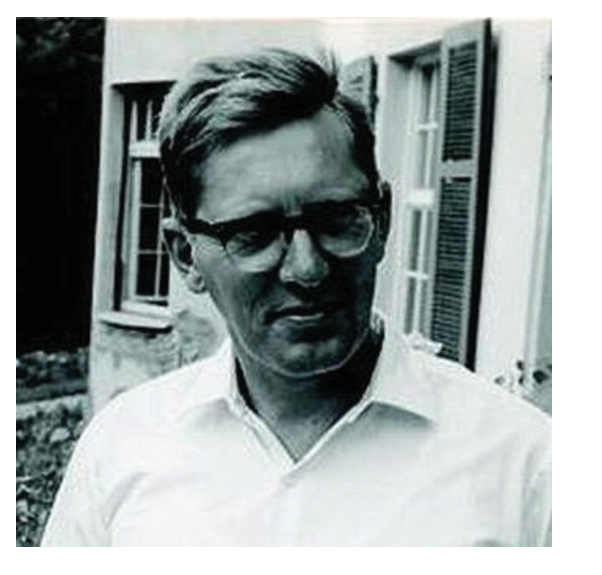
\includegraphics[width=2.0cm]{Bruijn.eps}}\noindent Nicolaas Govert de Bruijn (1918--2012) was a Dutch mathematician, noted for his many contributions in the fields of analysis, number theory, combinatorics and logic. De Bruijn started his academic career as at the University of Amsterdam, where he was Professor of Mathematics from 1952 to 1960. In 1960 he moved to the Technical University Eindhoven where he was Professor of Mathematics until his retirement in 1984.
In 1957 he was appointed member of the Royal Netherlands Academy of Arts and Sciences. He was Knighted with the Order of the Netherlands Lion.} coined the word \textit{multiset} in the 1970s. However, the use of multisets predates the word multiset by many centuries. The first study of multisets is usually attributed to an Indian mathematician who described permutations of multisets around 1150. In history, other names that were proposed or used for multisets include \textit{list}, \textit{bunch}, \textit{bag}, \textit{heap}, \textit{sample}, \textit{weighted set}, \textit{collection}, and \textit{suite}. The word ``visa'' is also used.

In the explicit form, multisets appeared in the work of \underline{Richard Dedekind}. Other mathematicians formalized multisets and began to study them as a precise mathematical object (structure) in the 20th century.

The multiplicity of an element is the number of instances of the element in a specific multiset. For example, an infinite number of multisets exist which contain only elements $a$ and $b$, varying only by multiplicity: The unique set $\{a, b\}$ contains only elements $a$ and $b$, each having multiplicity 1. In multiset $\{a, a, b\}$, $a$ has multiplicity 2 and $b$ has multiplicity 1.
In multiset $\{a, a, a, b, b, b\}$, $a$ and $b$ both have multiplicity 3.

\begin{definition}
Let $A$ be an ordinary set. A multiset $\alpha$ is a mapping from $A$ to $\mathbb{N}$ that gives the multiplicity of an element $a\in{A}$, denoted by $\alpha(a)$, representing the number of appearances of an element $a$ in $\alpha$. The cardinality of $\alpha$ is defined as $\sum_{a\in{A}}\alpha(a)$.
\end{definition}

By the definition, a multiset $\alpha$, given the underlying set $A$, can be written as $\alpha=\sum_{a\in{A}}\alpha(a).a$.

\begin{example}
In a multiset $\alpha=\{a, a, b, c, c, c\}$ on set $A=\{a, b, c, d\}$. We have $\alpha(a)=2$, $\alpha(b)=1$, $\alpha(c)=3$, and $\alpha(d)=0$. Then, the cardinality of $\alpha$, denoted as $|\alpha|$, is $\alpha(a)+\alpha(b)+\alpha(c)=6$. Write $\alpha=2a+b+3c$. For $x\in{A}$, If $\alpha(x)>0$, write $x\in\alpha$.
\end{example}

\begin{definition}
Let $\alpha$ and $\alpha^\prime$ be two multisets over a set $A$. Their addition, scalar multiplication, cover and substraction are defined as follows:

\begin{itemize}
  \item Addition: $\alpha+\alpha^\prime=_{\text{def}}\sum_{a\in{A}}(\alpha(a)+\alpha^\prime(a)).a$.
  \item Scalar multiplication: $n\times\alpha=_{\text{def}}\sum_{a\in{A}}(n\times\alpha(a)).a, n\in\mathbb{N}$.
  \item $\alpha$ covers $\alpha^\prime$: $\alpha\geq\alpha^\prime=_{\text{def}}\alpha(a)\geq\alpha^\prime(a), \forall a\in{A}$.
  \item $\alpha$ properly covers $\alpha^\prime$: $\alpha>\alpha^\prime=_{\text{def}}\alpha\geq\alpha^\prime$ and $\exists a\in{A}$, $\alpha(a)>\alpha^\prime(a)$.
  \item Substraction: $\alpha-\alpha^\prime=_{\text{def}}\sum_{a\in{A}}(\alpha(a)-\alpha^\prime(a)).a$ if $\alpha\geq\alpha^\prime$.
\end{itemize}
\end{definition}


\begin{definition}
A multiset $\alpha^\prime$ is said to be a subset of the multiset $\alpha$ if $\alpha\geq\alpha^\prime$. The power set of a multiset $\alpha$ (denoted as $2^\alpha$) is the set of all subsets of $\alpha$. If $\forall a\in{A}$, $\alpha(a)=0$, $\alpha$ is said to be an empty multiset. An empty multiset is usually written as $\emptyset$. We stipulate that $\emptyset\in 2^\alpha$ for any multiset $\alpha$.
\end{definition}

\begin{example}
Let $\alpha_1=2a+3b+c$ and $\alpha_2=a+2b$ be two multisets defined on a set $A=\{a, b, c, d\}$. We have $\alpha_1+\alpha_2=3a+5b+c$, $3\alpha_1=6a+9b+3c$, $\alpha_1\geq\alpha_2$, and $\alpha_1-\alpha_2=a+b+c$. Note that $2^{\alpha_2}=\{\emptyset, a, b, 2b, a+b, a+2b\}$. \hfill$\square$
\end{example}



\newpage
\section{Section Heading}
\label{sec:1}
Use the template \emph{chapter.tex} together with the Springer document class SVMono (monograph-type books) or SVMult (edited books) to style the various elements of your chapter content in the Springer layout.

\section{Section Heading}
\label{sec:2}
% Always give a unique label
% and use \ref{<label>} for cross-references
% and \cite{<label>} for bibliographic references
% use \sectionmark{}
% to alter or adjust the section heading in the running head
Instead of simply listing headings of different levels we recommend to let every heading be followed by at least a short passage of text. Furtheron please use the \LaTeX\ automatism for all your cross-references and citations.

Please note that the first line of text that follows a heading is not indented, whereas the first lines of all subsequent paragraphs are.

Use the standard \verb|equation| environment to typeset your equations, e.g.
%
\begin{equation}
a \times b = c\;,
\end{equation}
%
however, for multiline equations we recommend to use the \verb|eqnarray|
environment\footnote{In physics texts please activate the class option \texttt{vecphys} to depict your vectors in \textbf{\itshape boldface-italic} type - as is customary for a wide range of physical subjects.}.
\begin{eqnarray}
a \times b = c \nonumber\\
\vec{a} \cdot \vec{b}=\vec{c}
\label{eq:01}
\end{eqnarray}

\subsection{Subsection Heading}
\label{subsec:2}
Instead of simply listing headings of different levels we recommend to let every heading be followed by at least a short passage of text. Furtheron please use the \LaTeX\ automatism for all your cross-references\index{cross-references} and citations\index{citations} as has already been described in Sect.~\ref{sec:2}.

\begin{quotation}
Please do not use quotation marks when quoting texts! Simply use the \verb|quotation| environment -- it will automatically render Springer's preferred layout.
\end{quotation}


\subsubsection{Subsubsection Heading}
Instead of simply listing headings of different levels we recommend to let every heading be followed by at least a short passage of text. Furtheron please use the \LaTeX\ automatism for all your cross-references and citations as has already been described in Sect.~\ref{subsec:2}, see also Fig.~\ref{fig:1}\footnote{If you copy text passages, figures, or tables from other works, you must obtain \textit{permission} from the copyright holder (usually the original publisher). Please enclose the signed permission with the manucript. The sources\index{permission to print} must be acknowledged either in the captions, as footnotes or in a separate section of the book.}

Please note that the first line of text that follows a heading is not indented, whereas the first lines of all subsequent paragraphs are.

% For figures use
%
\begin{figure}[b]
\sidecaption
% Use the relevant command for your figure-insertion program
% to insert the figure file.
% For example, with the option graphics use
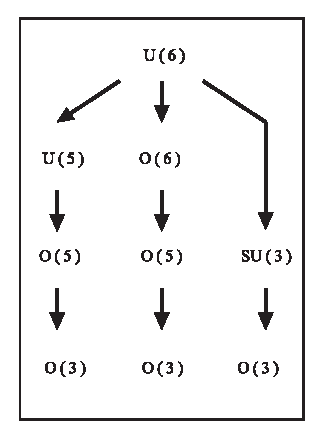
\includegraphics[scale=.65]{figure}
%
% If not, use
%\picplace{5cm}{2cm} % Give the correct figure height and width in cm
%
\caption{If the width of the figure is less than 7.8 cm use the \texttt{sidecapion} command to flush the caption on the left side of the page. If the figure is positioned at the top of the page, align the sidecaption with the top of the figure -- to achieve this you simply need to use the optional argument \texttt{[t]} with the \texttt{sidecaption} command}
\label{fig:1}       % Give a unique label
\end{figure}


\paragraph{Paragraph Heading} %
Instead of simply listing headings of different levels we recommend to let every heading be followed by at least a short passage of text. Furtheron please use the \LaTeX\ automatism for all your cross-references and citations as has already been described in Sect.~\ref{sec:2}.

Please note that the first line of text that follows a heading is not indented, whereas the first lines of all subsequent paragraphs are.

For typesetting numbered lists we recommend to use the \verb|enumerate| environment -- it will automatically render Springer's preferred layout.

\begin{enumerate}
\item{Livelihood and survival mobility are oftentimes coutcomes of uneven socioeconomic development.}
\begin{enumerate}
\item{Livelihood and survival mobility are oftentimes coutcomes of uneven socioeconomic development.}
\item{Livelihood and survival mobility are oftentimes coutcomes of uneven socioeconomic development.}
\end{enumerate}
\item{Livelihood and survival mobility are oftentimes coutcomes of uneven socioeconomic development.}
\end{enumerate}


\subparagraph{Subparagraph Heading} In order to avoid simply listing headings of different levels we recommend to let every heading be followed by at least a short passage of text. Use the \LaTeX\ automatism for all your cross-references and citations as has already been described in Sect.~\ref{sec:2}, see also Fig.~\ref{fig:2}.

Please note that the first line of text that follows a heading is not indented, whereas the first lines of all subsequent paragraphs are.

For unnumbered list we recommend to use the \verb|itemize| environment -- it will automatically render Springer's preferred layout.

\begin{itemize}
\item{Livelihood and survival mobility are oftentimes coutcomes of uneven socioeconomic development, cf. Table~\ref{tab:1}.}
\begin{itemize}
\item{Livelihood and survival mobility are oftentimes coutcomes of uneven socioeconomic development.}
\item{Livelihood and survival mobility are oftentimes coutcomes of uneven socioeconomic development.}
\end{itemize}
\item{Livelihood and survival mobility are oftentimes coutcomes of uneven socioeconomic development.}
\end{itemize}

\begin{figure}[t]
\sidecaption[t]
% Use the relevant command for your figure-insertion program
% to insert the figure file.
% For example, with the option graphics use
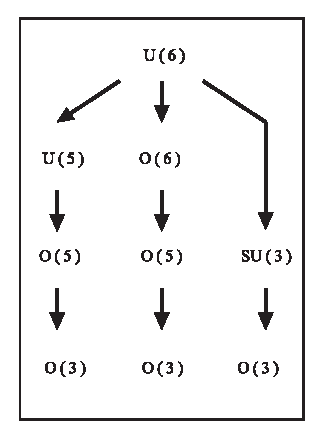
\includegraphics[scale=.65]{figure}
%
% If not, use
%\picplace{5cm}{2cm} % Give the correct figure height and width in cm
%
\caption{Please write your figure caption here}
\label{fig:2}       % Give a unique label
\end{figure}

\runinhead{Run-in Heading Boldface Version} Use the \LaTeX\ automatism for all your cross-references and citations as has already been described in Sect.~\ref{sec:2}.

\subruninhead{Run-in Heading Italic Version} Use the \LaTeX\ automatism for all your cross-refer\-ences and citations as has already been described in Sect.~\ref{sec:2}\index{paragraph}.
% Use the \index{} command to code your index words
%
% For tables use
%
\begin{table}
\caption{Please write your table caption here}
\label{tab:1}       % Give a unique label
%
% For LaTeX tables use
%
\begin{tabular}{p{2cm}p{2.4cm}p{2cm}p{4.9cm}}
\hline\noalign{\smallskip}
Classes & Subclass & Length & Action Mechanism  \\
\noalign{\smallskip}\svhline\noalign{\smallskip}
Translation & mRNA$^a$  & 22 (19--25) & Translation repression, mRNA cleavage\\
Translation & mRNA cleavage & 21 & mRNA cleavage\\
Translation & mRNA  & 21--22 & mRNA cleavage\\
Translation & mRNA  & 24--26 & Histone and DNA Modification\\
\noalign{\smallskip}\hline\noalign{\smallskip}
\end{tabular}
$^a$ Table foot note (with superscript)
\end{table}
%
\section{Section Heading}
\label{sec:3}
% Always give a unique label
% and use \ref{<label>} for cross-references
% and \cite{<label>} for bibliographic references
% use \sectionmark{}
% to alter or adjust the section heading in the running head
Instead of simply listing headings of different levels we recommend to let every heading be followed by at least a short passage of text. Furtheron please use the \LaTeX\ automatism for all your cross-references and citations as has already been described in Sect.~\ref{sec:2}.

Please note that the first line of text that follows a heading is not indented, whereas the first lines of all subsequent paragraphs are.

If you want to list definitions or the like we recommend to use the Springer-enhanced \verb|description| environment -- it will automatically render Springer's preferred layout.

\begin{description}[Type 1]
\item[Type 1]{That addresses central themes pertainng to migration, health, and disease. In Sect.~\ref{sec:1}, Wilson discusses the role of human migration in infectious disease distributions and patterns.}
\item[Type 2]{That addresses central themes pertainng to migration, health, and disease. In Sect.~\ref{subsec:2}, Wilson discusses the role of human migration in infectious disease distributions and patterns.}
\end{description}

\subsection{Subsection Heading} %
In order to avoid simply listing headings of different levels we recommend to let every heading be followed by at least a short passage of text. Use the \LaTeX\ automatism for all your cross-references and citations citations as has already been described in Sect.~\ref{sec:2}.

Please note that the first line of text that follows a heading is not indented, whereas the first lines of all subsequent paragraphs are.

\begin{svgraybox}
If you want to emphasize complete paragraphs of texts we recommend to use the newly defined Springer class option \verb|graybox| and the newly defined environment \verb|svgraybox|. This will produce a 15 percent screened box 'behind' your text.

If you want to emphasize complete paragraphs of texts we recommend to use the newly defined Springer class option and environment \verb|svgraybox|. This will produce a 15 percent screened box 'behind' your text.
\end{svgraybox}


\subsubsection{Subsubsection Heading}
Instead of simply listing headings of different levels we recommend to let every heading be followed by at least a short passage of text. Furtheron please use the \LaTeX\ automatism for all your cross-references and citations as has already been described in Sect.~\ref{sec:2}.

Please note that the first line of text that follows a heading is not indented, whereas the first lines of all subsequent paragraphs are.

\begin{theorem}
Theorem text goes here.
\end{theorem}
%
% or
%
\begin{definition}
Definition text goes here.
\end{definition}

\begin{proof}
%\smartqed
Proof text goes here.
\qed
\end{proof}

\paragraph{Paragraph Heading} %
Instead of simply listing headings of different levels we recommend to let every heading be followed by at least a short passage of text. Furtheron please use the \LaTeX\ automatism for all your cross-references and citations as has already been described in Sect.~\ref{sec:2}.

Note that the first line of text that follows a heading is not indented, whereas the first lines of all subsequent paragraphs are.
%
% For built-in environments use
%
\begin{theorem}
Theorem text goes here.
\end{theorem}
%
\begin{definition}
Definition text goes here.
\end{definition}
%
\begin{proof}
\smartqed
Proof text goes here.
\qed
\end{proof}
%
\begin{acknowledgement}
If you want to include acknowledgments of assistance and the like at the end of an individual chapter please use the \verb|acknowledgement| environment -- it will automatically render Springer's preferred layout.
\end{acknowledgement}
%
\section*{Appendix}
\addcontentsline{toc}{section}{Appendix}
%
When placed at the end of a chapter or contribution (as opposed to at the end of the book), the numbering of tables, figures, and equations in the appendix section continues on from that in the main text. Hence please \textit{do not} use the \verb|appendix| command when writing an appendix at the end of your chapter or contribution. If there is only one the appendix is designated ``Appendix'', or ``Appendix 1'', or ``Appendix 2'', etc. if there is more than one.

\begin{equation}
a \times b = c
\end{equation}
% Problems or Exercises should be sorted chapterwise
\section*{Problems}
\addcontentsline{toc}{section}{Problems}
%
% Use the following environment.
% Don't forget to label each problem;
% the label is needed for the solutions' environment
\begin{prob}
\label{prob1}
A given problem or Excercise is described here. The
problem is described here. The problem is described here.
\end{prob}

\begin{prob}
\label{prob2}
\textbf{Problem Heading}\\
(a) The first part of the problem is described here.\\
(b) The second part of the problem is described here.
\end{prob}

%\input{referenc_1}

\begin{thebibliography}{99}


\bibitem{Lipschutz2007}
S. Lipschutz and M. L. Lipson, \textit{Schaum's Outline of Theory and Problems of Discrete Mathematics}, Third Edition, New York: McGraw-Hill, 2007.

\bibitem{Rosen2007}
K. H. Rosen, \textit{Discrete Mathematics and Its Applications}, Seventh Edition, New York: McGraw-Hill, 2007.

\bibitem{Maclane1988}
S. Maclane and G. Birkhoff, \textit{Algebra}, Third Edition, New York: Bchelsea Publishing Company, 1988.
\end{thebibliography}

%\include{chapter_21}
%\include{chapter_2_function}
%%%%%%%%%%%%%%%%%%%%%% appendix.tex %%%%%%%%%%%%%%%%%%%%%%%%%%%%%%%%%
%
% sample appendix
%
% Use this file as a template for your own input.
%
%%%%%%%%%%%%%%%%%%%%%%%% Springer-Verlag %%%%%%%%%%%%%%%%%%%%%%%%%%

\appendix
\motto{All's well that ends well}
\chapter{Chapter Heading}
\label{introA} % Always give a unique label
% use \chaptermark{}
% to alter or adjust the chapter heading in the running head

Use the template \emph{appendix.tex} together with the Springer document class SVMono (monograph-type books) or SVMult (edited books) to style appendix of your book in the Springer layout.


\section{Section Heading}
\label{sec:A1}
% Always give a unique label
% and use \ref{<label>} for cross-references
% and \cite{<label>} for bibliographic references
% use \sectionmark{}
% to alter or adjust the section heading in the running head
Instead of simply listing headings of different levels we recommend to let every heading be followed by at least a short passage of text. Furtheron please use the \LaTeX\ automatism for all your cross-references and citations.


\subsection{Subsection Heading}
\label{sec:A2}
Instead of simply listing headings of different levels we recommend to let every heading be followed by at least a short passage of text. Furtheron please use the \LaTeX\ automatism for all your cross-references and citations as has already been described in Sect.~\ref{sec:A1}.

For multiline equations we recommend to use the \verb|eqnarray| environment.
\begin{eqnarray}
\vec{a}\times\vec{b}=\vec{c} \nonumber\\
\vec{a}\times\vec{b}=\vec{c}
\label{eq:A01}
\end{eqnarray}

\subsubsection{Subsubsection Heading}
Instead of simply listing headings of different levels we recommend to let every heading be followed by at least a short passage of text. Furtheron please use the \LaTeX\ automatism for all your cross-references and citations as has already been described in Sect.~\ref{sec:A2}.

Please note that the first line of text that follows a heading is not indented, whereas the first lines of all subsequent paragraphs are.

% For figures use
%
\begin{figure}[t]
\sidecaption[t]
%\centering
% Use the relevant command for your figure-insertion program
% to insert the figure file.
% For example, with the option graphics use
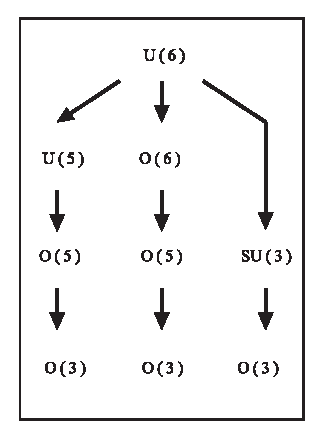
\includegraphics[scale=.65]{figure}
%
% If not, use
%\picplace{5cm}{2cm} % Give the correct figure height and width in cm
%
\caption{Please write your figure caption here}
\label{fig:A1}       % Give a unique label
\end{figure}

% For tables use
%
\begin{table}
\caption{Please write your table caption here}
\label{tab:A1}       % Give a unique label
%
% For LaTeX tables use
%
\begin{tabular}{p{2cm}p{2.4cm}p{2cm}p{4.9cm}}
\hline\noalign{\smallskip}
Classes & Subclass & Length & Action Mechanism  \\
\noalign{\smallskip}\hline\noalign{\smallskip}
Translation & mRNA$^a$  & 22 (19--25) & Translation repression, mRNA cleavage\\
Translation & mRNA cleavage & 21 & mRNA cleavage\\
Translation & mRNA  & 21--22 & mRNA cleavage\\
Translation & mRNA  & 24--26 & Histone and DNA Modification\\
\noalign{\smallskip}\hline\noalign{\smallskip}
\end{tabular}
$^a$ Table foot note (with superscript)
\end{table}
%


%\backmatter%%%%%%%%%%%%%%%%%%%%%%%%%%%%%%%%%%%%%%%%%%%%%%%%%%%%%%%
%\include{glossary}
%
\Extrachap{Solutions}

\section*{Problems of Chapter~\ref{intro}}

\begin{sol}{prob1}
The solution\index{problems}\index{solutions} is revealed here.
\end{sol}


\begin{sol}{prob2}
\textbf{Problem Heading}\\
(a) The solution of first part is revealed here.\\
(b) The solution of second part is revealed here.
\end{sol}


%\printindex

%%%%%%%%%%%%%%%%%%%%%%%%%%%%%%%%%%%%%%%%%%%%%%%%%%%%%%%%%%%%%%%%%%%%%%

$\emph{P}$ $\texttt{P}$ $\P$  $\mathrm{P}$  $\mathcal{P}$ $\mathit{P}$  $\mathnormal{P}$  $\boldsymbol{P}$  $\mathbf{P}$

中文示例

\begin{myTh}
	content...
\end{myTh}

$\notin\beta$

\begin{myTh}
	
\end{myTh}

\begin{myDf}
	
\end{myDf}

\hfill

$\textbf{the signatures of the transition relations:}$

$T \in \mathbb{P}(Q \times V \times Q)$

$T \in V \to P(Q \times Q)$

$T \in Q\times Q \to P(V)$

$T \in Q \times V \to P(Q)$

$T \in Q \to P(V \times Q)$

for example, the function $T \in Q \to P(V \times Q)$ is defined as $T(p) = \{(a,q):(p,a,q) \in T\}$

\hfill

$\textbf{$\epsilon$-transition relation:}$

$E \in P(Q\times Q)$

$E \in Q \to P(Q)$

\hfill

$T \in P(Q \times V \times Q), T = \{(s,a,q) \}$

$T(s)\in Q \to P(V\times Q), T(s) = \{(a,q):(s,a,q) \in T\}$

$Q_{map}: P(Q\times V), Q_{map} = \{(q,a): (s,a,q) \in T\}$

$Q_{map}(q) = \{a: (s,a,q)\in T\}$

${Q_{map}}^{-1}: V \nrightarrow P(Q), {Q_{map}}^{-1} = \{(a,q): (s,a,q) \in T\}$

According to Convention A.4 (Tuple projection):

$\bar{\pi}_2(T) = \{(s,q): (s,a,q)\in T \}$

$Q_{map} = (\bar{\pi}_1(T))^R, Q_{map} = \{(a,q):(s,a,q) \in T\}^R = \{(q,a):(s,a,q) \in T\}$

\hfill

$f(a)=(f(a^R))^R$

\hfill

$\textbf{Prefix-closure:}$ Let $L\subseteq V^*$,then
$$\overline{L} := \{s\in V^*:(\exists t\in V^*)[st\in L]\}$$

In words, the prefix closure of L is the language denoted by $\overline{L}$ and consisting of all the prefixes in L. In general, $L\subseteq \overline{L}$.

L is said to be prefix-closed if $L = \overline{L}$. Thus language L is prefix-closed if any prefix of any string in L is also an element of L.

$L_1 = \{\epsilon,a,aa\}, L_1 = \overline{L_1}, L_{1}$ is prefix-closed.

$L_2 = \{a,b,ab\}, \overline{L_2} = \{\epsilon,a,b,ab\}, L_2 \subset \overline{L_2}, L_2$ is not prefix closed.

\hfill

$\textbf{Post-language:}$ Let $L\subseteq V^{\ast}$ and $s\in L$. Then the post-language of L after s, denoted by L/s, is the language
$$ L/s := \{t\in V^{\ast}:st\in L\}$$
By definition, $L/s = \emptyset$ if $s \notin \overline{L}$.

\hfill

\begin{myDf}[Left derivatives]: Given language $A\subseteq V^{\ast}$ and $w\in V^{\ast}$ we define the left derivative of A with respect to $w$ as:
$$w^{-1}A = \{x\in V^{\ast}:wx\in A\}$$
$A$关于$w$的左导数,就是$A$中: \{$w$的后缀组成的字符串集合\}。

Sometimes derivatives are written as $D_{w}A$ or as $\frac{dA}{dw}$. Right derivatives are analogously defined. Derivatives can also be extended to $B^{-1}A$ where B is also a language.
\end{myDf}

\begin{myExt}
$A = \{a,aab,baa\},a^{-1}A = D_{a}A = \frac{dA}{da} =\{\epsilon,ab,\emptyset\} = \{\epsilon,ab\}$
\end{myExt}

\begin{myExt}
	$L = \{ba,baa,baab,ca\}, w = \{ba\},$
	
	$w^{-1}L =\{\epsilon,a,ab,\emptyset\} = \{\epsilon,a,ab\}$
	
	${(wa)}^{-1}L = {(baa)}^{-1}L = \{\emptyset,\epsilon,b,\emptyset\} = \{\epsilon,b\}$
	
	$a^{-1}(w^{-1}L) = a^{-1}\{\epsilon,a,ab\} = \{\emptyset,\epsilon,b\} = \{\epsilon,b\}$
	
	$w\in L \equiv \epsilon \in w^{-1}L,and {(wa)}^{-1}L = a^{-1}(w^{-1}L)$
\end{myExt}

\begin{myExt}
	$a^{-1}\{a\} = \{\epsilon\}; \quad a^{-1}\{b\} = \emptyset,\quad\Leftarrow if (a\ne b)$
\end{myExt}

\begin{myExt}
	$L_0 = \{ab\},L_1 = \{ac\}, L_0L_1 = \{abac\}$
	
	$a^{-1}(L_0L_1) = \{bac\}$
	
	$a^{-1}(L_0L_1) = (a^{-1}L_0)L_1 \cup \emptyset \quad \Leftarrow(\epsilon \notin L_0)$
	
	$= \{b\}L_1 = \{bac\}$
\end{myExt}

\begin{myExt}
	$L_0 = \{\epsilon,ab\},L_1 = \{ac\}, L_0L_1 = \{ac,abac\}$
	
	$a^{-1}(L_0L_1) = \{c,bac\}$
	
	$a^{-1}(L_0L_1) = (a^{-1}L_0)L_1 \cup a^{-1}L_1 \quad\Leftarrow(\epsilon \in L_0)$
	
	$= \{\emptyset,b\}L_1 \cup \{c\} = \{c,bac\}$
\end{myExt}

\begin{myPf}
	$a^{-1}(L_0L_1)$
	
	$1. if(\epsilon \in L_0) \Rightarrow a^{-1}(L_0L_1) = (a^{-1}L_0)L_1 \cup a^{-1}L_1 $ 
	
	$L_0 = (L_0 \backslash \{\epsilon\}) \cup \{\epsilon\}$
	
	$a^{-1}(L_0L_1) = a^{-1}(((L_0 \backslash \{\epsilon\}) \cup \{\epsilon\})L_1)$
	
	$=a^{-1}(L_0L_1\cup L_1)$
	
	$a^{-1}L_0 = a^{-1}((L_0 \backslash \{\epsilon\}) \cup \{\epsilon\})$
	
	$=a^{-1}(L_0\ \backslash \{\epsilon \}) \cup a^{-1}\{\epsilon \}$
	
	$=a^{-1}L_0 \cup \emptyset = a^{-1}L_0$
\end{myPf}
	

\clearpage

自动机理论、语言和计算机导论,P99

(1)如果$L$是一个语言,$a$是一个符号,则$L/a$(称作$L$和$a$的商)是所有满足如下条件的串$w$的集合:$wa$属于$L$。
例如,如果$L=\{a,aab,baa\}$,则$L/a = \{\epsilon,ba\}$, 证明:如果$L$是正则的,那么$L/a$也是。提示:从$L$的$DFA$出发,考虑接受状态的集合。

(2)如果$L$是一个语言,$a$是一个符号,则$a\backslash L$是所有满足如下条件的串$w$的集合: $aw$属于$L$。例如,如果$L=\{a,aab,baa\}$,则$a\backslash L=\{\epsilon,ab\}$,证明:如果$L$是正则的,那么$a\backslash L$也是。提示:记得正则语言在反转运算下是封闭的,又由(1)知,正则语言的商运算下是封闭的。

\begin{myDf}[Kleene-closure]: 
	Let $L\subseteq V^{\ast}$, then 
	$$L^{\ast} := \{\epsilon\}\cup L \cup LL\cup LLL\cup \cdots$$ 
\end{myDf}

This is the same operation that we defined above for the set V, except that now it is applied to set L whose elements may be strings of length greater than one. An element of $L^*$ is formed by the concatenation of a finite (but possibly arbitrarily large) number of elements of L; this includes the concatenation of "zero" elements, that is the empty string $\epsilon$. Note that $\ast$ operation is idempotent: ${(L^*)}^* = L^*$.
\begin{align*}
L^{\ast} & = (L\backslash \{\epsilon\})L^{\ast}\cup \{\epsilon\} \\
         & = \{\epsilon \} \cup L\cup LL\cup LLL\cup \dots
\end{align*}




\end{document}

